\chapter{Parameterized Token Rings} \label{chap:token-systems}

\newcommand\VarNames{\textsf{Vars}}
\newcommand{\pring}{\ensuremath{\mathcal {R}}}
\renewcommand{\trans}[3]{#1 \stackrel{{#3}}{\rightarrow} #2}
\newcommand{\trcv}{\mathsf{rcv}}
\newcommand{\tsnd}{\mathsf{snd}}
\newcommand{\sch}{\mathsf{sch}}
\newcommand{\token}{\mathsf{tok}}
\newcommand{\powerset}[1]{2^{#1}}
\newcommand{\Locals}{Q}
\newcommand{\LocalsI}{\Locals_0}
\newcommand{\ActionsProc}{\Sigma_{\mathsf{pr}}}
%\newcommand{\ActionsSys}{\Sigma_{\mathsf{sys}}}

\newcommand{\IndSet}{\bbN}

\newcommand{\Opr}{{\mathrm{O}_{\mathrm{pr}}}}
\newcommand{\Osys}{{\mathrm{O}_{\mathrm{sys}}}}

% \newcommand{\Ipr}{{\mathrm{I}_{\mathrm{int}}}}
\newcommand{\IprAll}{{\mathrm{I}_{\mathrm{pr}}}}
\newcommand{\Iloc}{\mathrm{I}_{loc}}
\newcommand{\Iglob}{\mathrm{I}_{glob}}
\newcommand{\Ipr}{\IprAll}
\newcommand{\Isys}{{\mathrm{I}_{\mathrm{sys}}}}

% AMBA signals
\newcommand{\ambasignal}[1]{\textsc{#1}}
\newcommand{\ambasignali}[2][i]{\textsc{#2}[\textrm{#1}]}
\newcommand{\hgrant}{\ambasignal{\textcolor{blue}{hgrant}}}
\newcommand{\hgranti}[1][i]{\ambasignali[#1]{\textcolor{blue}{hgrant}}}
\newcommand{\hbusreq}{\ambasignal{\textcolor{red}{hbusreq}}}
\newcommand{\hbusreqi}[1][i]{\ambasignali[#1]{\textcolor{red}{hbusreq}}}
\newcommand{\hready}{\ambasignal{\textcolor{red}{hready}}}
\newcommand{\hreadyi}[1][i]{\ambasignali[#1]{\textcolor{red}{ready}}}
\newcommand{\hlock}{\ambasignal{\textcolor{red}{hlock}}}
% \newcommand{\hlocki}[1][i]{\ambasignali[#1]{hlock}}
\newcommand{\hlocki}{\ambasignali[i]{\textcolor{red}{hlock}}}
\newcommand{\hmastlock}{\ambasignal{\textcolor{blue}{hmastlock}}}
\newcommand{\hmastlocki}[1][i]{\ambasignali[#1]{\textcolor{blue}{hmastlock}}}
\newcommand{\hburst}{\ambasignal{\textcolor{red}{hburst}}}
\newcommand{\hbursti}{\ambasignali[i]{\textcolor{red}{hburst}}}
% \newcommand{\hbursti}[1][i]{\ambasignali[#1]{hburst}}
\newcommand{\hmaster}{\ambasignal{\textcolor{blue}{hmaster}}}
\newcommand{\hmasteri}[1][i]{\ambasignali[#1]{\textcolor{blue}{hmaster}}}
\newcommand{\hstart}{\ambasignal{\textcolor{blue}{start}}}
\newcommand{\hstarti}[1][i]{\ambasignali[#1]{\textcolor{blue}{start}}}
\newcommand{\hlocked}{\ambasignal{\textcolor{blue}{locked}}}
\newcommand{\hlockedi}[1][i]{\ambasignali[#1]{\textcolor{blue}{locked}}}
\newcommand{\hdecide}{\ambasignal{\textcolor{blue}{decide}}}
% \newcommand{\hdecidei}[1][i]{\ambasignali[i]{decide}}
\newcommand{\hdecidei}{\ambasignali[i]{\textcolor{blue}{decide}}}
\newcommand{\tok}{\ambasignal{\textcolor{blue}{tok}}}
% \newcommand{\toki}[1][i]{\ambasignali[#1]{tok}}
\newcommand{\toki}{\ambasignali[i]{\textcolor{blue}{tok}}}
\newcommand{\hincr}{\ambasignal{incr}}
\newcommand{\hburstfour}{\ambasignal{burst4}}
\newcommand{\hburstthree}{\ambasignal{burst3}}
\newcommand{\norequestsi}{\ambasignali{\textcolor{red}{no\_req}}}
\newcommand{\norequests}{\ambasignal{\textcolor{red}{no\_req}}}
\newcommand{\send}{\ambasignal{send}}
\newcommand{\sendi}{\ambasignali[i]{send}}

\hfill {\footnotesize\textit{This chapter is based on joint work with R.Bloem and S.Jacobs~\cite{Khalimov13,party,BJK14}}~~~~~~~~}

\begin{quotation}
\noindent\textbf{Abstract.}
Parameterized synthesis was recently proposed as a way
to circumvent the poor scalability of current synthesis tools.
The method uses cutoff results in token rings to
reduce the problem to bounded distributed synthesis,
and ultimately to a sequence of SMT problems. 
But experiments show that the size of the specification is a major issue. 
In this chapter we
 (1) propose several optimizations of the approach, and
 (2) perform a parameterized synthesis case study on the industrial arbiter protocol AMBA.

In the first part of this chapter,
we optimize the reduction of the parameterized to distributed synthesis.
To this end,
we refine the cutoff reduction using modularity and abstraction.
The evaluation, using our specially developed parameterized synthesizer PARTY,
shows that the optimizations lead to several orders of magnitude speed-ups.

In the second part, we perform parameterized synthesis case study
on the industrial arbiter protocol AMBA.
The AMBA protocol has been used as a benchmark for many reactive synthesis tools,
because it is hard to synthesize an implementation that can serve a large number of clients.
We show how to use parameterized synthesis to obtain a component that serves a single master,
and can be arranged in a ring of arbitrarily many components.
We describe new tricks---a cutoff extension tailored for AMBA and decompositional synthesis---%
that together with the previously described optimizations allowed us
to synthesize a component with 14 states in about 1 hour.
\end{quotation}

\section{Introduction}

By automatically generating correct implementations from a temporal logic 
specification, reactive synthesis tools can relieve system designers from 
tedious and error-prone tasks like low-level manual implementation and 
debugging. This great benefit comes at the cost of high computational complexity 
of synthesis, which makes synthesis of large systems an ambitious goal. 
For instance, Bloem et al.~\cite{Bloem12}
synthesize an arbiter for the ARM AMBA Advanced High
Performance Bus (AHB)~\cite{AMBAspec}. The results, obtained using 
RATSY~\cite{Bloem10c},
show that both the size of the implementation and the time for synthesis
increase steeply with the number of masters that the arbiter can
handle. This is unexpected, since an arbiter for $n+1$ masters is very 
similar to an arbiter for $n$ masters, and manual implementations grow only 
slightly with the number of masters. While recent results show that 
synthesis time and implementation size can be improved in standard LTL 
synthesis tools~\cite{BS,GodhalCH13}, the fundamental problem of increasing 
complexity with the number of masters can only be solved by adapting the 
synthesis approach itself.

To this end, Jacobs and Bloem~\cite{JB14} introduced the 
\emph{parameterized synthesis} approach.
A simple example of a parameterized specification is the following LTL specification of a simple arbiter:
\[ \begin{array}{ll}
  \forall i \neq j.~ & \G \neg ( g_i \land g_j ) \land \\
  \forall i.~ & \G (r_i \impl \F g_i).
  \end{array}
\]
In parameterized synthesis, we synthesize a building block that can be cloned to form a system that satisfies such a specification, for any number of components.

Jacobs and Bloem~\cite{JB14} showed that parameterized synthesis is undecidable in general, but semi-decision procedures can be found for classes of systems with cutoffs, i.e., where parameterized verification can be reduced to verification of a system with a bounded number of components. They presented a semi-decision procedure for token-ring networks, building on results by Emerson and Namjoshi~\cite{Emerso03}, which show that for the verification of parameterized token rings, a cutoff of $5$ is sufficient for a certain class of specifications. Following these results, parameterized synthesis reduces to distributed synthesis in token rings of (up to) $5$ identical processes. To solve the resulting problem, a modification of the SMT encoding of the distributed bounded synthesis problem by Finkbeiner and Schewe~\cite{BS} was used.

Experiments with the parameterized synthesis method~\cite{JB14} revealed that only very small specifications could be handled with this encoding. For example, the simple arbiter presented before can be synthesized in a few seconds for a ring of size $4$, which is the sufficient cutoff for this specification. However, synthesis does not terminate within $2$ hours for a specification that also excludes spurious grants, in a ring of the same size. Furthermore, the previously proposed method uses cutoff results of Emerson and Namjoshi~\cite{Emerso03} and therefore inherits a restricted language support and cannot handle specifications in assume-guarantee style~\cite{Bloem12}.
This precludes the approach from being applied to the AMBA protocol.

In this chapter we address both issues.

In the first part of the chapter (Section~\ref{tok_rings:sec:bs-and-optimizations}),
we optimize the reduction of the parameterized to distributed synthesis.
We use the fact that
(a) token-ring systems consist of isomorphic processes,
(b) different properties may require different cutoffs, and
(c) when model checking the behaviours of some fixed processes,
    the behaviours of the others can be abstracted.
The evaluation,
using our specially developed parameterized synthesizer PARTY,
show that the optimizations lead to several orders of magnitude speed-ups.
 
In the second part of the chapter (Section~\ref{amba:sec}),
we perform parameterized synthesis case study on the industrial arbiter protocol AMBA.
The AMBA protocol has been used as a benchmark for many reactive synthesis tools,
because it is hard to synthesize an implementation that can serve
a large number of clients. We show how to use parameterized synthesis
to obtain a component that serves a single master, and can be arranged
in a ring of arbitrarily many components.
We describe new tricks%
---a cutoff extension tailored for AMBA and decompositional synthesis---%
that together with the previously described optimizations allowed us
to synthesize a component with 14 states in about 1 hour.

The chapter starts with definitions in Section~\ref{tok_rings:defs},
where we introduce token-ring systems, parameterized specifications and problems.
Then we state known cutoff results and a slight generalization.
Section~\ref{tok_rings:sec:bs-and-optimizations} describes
the SMT encoding of the bounded synthesis for token-ring systems,
followed by optimizations and experiments.
Then we proceed to the AMBA case study (Section~\ref{amba:sec}).
We describe the protocol and its parameterized specification.
Section~\ref{amba:sec:handling-amba} contains the main contribution:
(1) we rewrite the specification into the form feasible to parameterized synthesis and
(2) we extend the known cutoffs to handle the resulting AMBA specification.
In Section~\ref{amba:sec:experiments} on experiments,
we describe the crucial optimization ``decompositional synthesis''
and report synthesis timings.

%%%%%%%%%%%%%%%%%%%%%%%%%%%%%%%%%%%%%%%%%%%%%%%%%%%%%%%%%%%%%%%%%%%%%%%%%%%%%%%%%%%%
\section{Definitions} \label{tok_rings:defs}

\subsection{Token-ring Systems} \label{tok_rings:defs:system}
In this section we define token ring systems---%
the LTS that consists of replicated copies of a process connected in a uni-directional ring.
Transitions in a token ring system are either internal or synchronized
(in which one process sends the token to the next process along the ring).
The token starts in a non-deterministically chosen process.

We start by recalling a (non-deterministic) labeled transition system.
A \emph{labeled transition system (LTS)}
is a tuple
$(I,O,Q,Q_0,\delta,out)$
where
 $I$ is the set of {\em inputs},
 $O$ is the set of {\em outputs} disjoint from $I$,
 $Q$ is the set of {\em states},
 $Q_0 \subseteq Q$ is the set of {\em initial states},
 $\delta \subseteq Q \times 2^I \times Q$ is the {\em transition relation},
 and $out:Q \to 2^O$ is the \emph{output function} (also called {\em state-labeling} function).

Fix two disjoint sets:
a set $\Opr$ of process template \emph{output variables} that contains two distinguished output variable,
$\tsnd$ and $\token$,
and a set $\Ipr$ of process template \emph{input variables} that contains a distinguished input variable $\trcv$.
We always assume that $\Ipr$ and $\Opr$ are disjoint.


\parbf{Process template} \label{page:tok_rings:defs:process_template}
A {\em process template} $P$ is an LTS
$(\Ipr, \Opr, Q, Q_0, \delta, out, A_{loc})$:
\begin{enumerate}[label*=\roman*)]
\item 
The state set $Q$ is finite and can be partitioned into two non-empty disjoint sets: $Q = T \cupdot NT$. 
    States in $T$ are said to {\em have the token}.

\item
The initial state set is $Q_0  = \{\iota_t, \iota_n\}$ for some $\iota_t \in T, \iota_n \in NT$.

\item
The output function is $out: Q \rightarrow 2^{\Opr}$ and it satisfies:
\li
\- for every $t \in NT$: $\token \not\in out(t)$ and for every $t \in T$: $\token \in out(t)$,
\- for every $t \in Q$: $\tsnd \in out(t) \impl t \in T$.
\il

\item
Let $\ActionsProc = 2^\Ipr$.
Let $\ActionsProc^\trcv = \{ i \in \ActionsProc \| \trcv \in i \}$, 
$\ActionsProc^{\neg \trcv} = \ActionsProc \setminus \Sigma^\trcv$,
$T^\tsnd = \{ q \in \Locals \| \tsnd \in out(q) \}$,
$T^{\neg \tsnd} = T \setminus T^\tsnd$.
Then the transition function: 
\begin{equation}\label{tok_rings:eq:process-trans}
\delta \subseteq 
T^\tsnd \times \ActionsProc^{\neg \trcv}\times NT  ~~\cup~~
NT\times\ActionsProc^\trcv\times T   ~~\cup~~
NT\times\ActionsProc^{\neg \trcv}\times NT   ~~\cup~~
T^{\neg \tsnd}\times\ActionsProc^{\neg \trcv}\times T.
\end{equation}

Also, $\delta$ is non-terminating: 
for every $q \in NT$ and every $i \in \ActionsProc$
  there exists $\trans{q}{q'}{i}$; 
and for every $q \in T$ and every $i \in \ActionsProc^{\neg \trcv}$
  there exists $\trans{q}{q'}{i}$.

\item [$\dagger$)]
$A_{loc}$ is a \emph{fairness} condition over $\Ipr \cup \Opr$.
We require that on every infinite path from an initial state and satisfying $A_{loc}$,
from any state with the token, $q \in T$, the process reaches a state $q'$ where it sends the token.
(In LTL this can be written as $A_{loc} \impl \G(\token \impl \F \tsnd)$.)
We call this requirement ($\dagger$).
We omit $A_{loc}$ in the LTS tuple when it is not important.
\end{enumerate}



\parbf{Ring topology $R$}
A {\em ring} is a directed graph $R = (V,E)$,
where the set of vertices is $V = \{ 1,\ldots,k\}$ for some $k \in \IndSet$,
and the set of edges is $E = \{(i,i_{mod |V|}+1) \mid i\in V\}$.
We will skip ``$mod |V|$'' and write $i+1$.
Vertices are called {\em process indices}.


\parbf{Token-ring system $P^R$}
Fix a ring topology $R=(V,E)$.

Let $\Isys = (\Iloc \times V) \cupdot \Iglob$
be the \emph{system input variables},
where local inputs $\Iloc$ and global inputs $\Iglob$ are
such that $\Ipr = \Iloc \cupdot \Iglob$.
%Define $\ActionsSys = \powerset{\Isys}$.
For system input ${\sf in} \in 2^\Isys$,
let ${\sf in}(v) = \{ i \in {\sf in} \| i\in \Iloc\times\{v\} \cup \Iglob \}$
denote the input to process $v$ (including global inputs).

Let $\Osys = \Opr \times V$ be the \emph{system output variables}. 
For $(p,i)$ in $\Osys$ or in $\Isys\setminus \Iglob$ we write $p_i$. 

Given a process template $P =  (\Ipr, \Opr, Q, Q_0, \delta, out)$
and a token ring topology $R = (V,E)$,
the {\em token-ring system} $P^R$ is the LTS $(\Isys,\Osys,S,S_0,\Delta,Out)$:

\li
\- The set $S$ of \emph{global states} is $Q^V$,
   i.e., all functions from $V$ to $Q$.
   If $s \in Q^V$ is a global state
   then $s(i)$ denotes the local state of the process with index $i$.

\- The set of \emph{global initial states} $S_0$ contains all $s_0 \in Q_0^V$
   in which exactly one of the processes has the token.

\- The labeling $Out(s): S \to 2^\Osys$ is:
   for every $s \in S$: $p_i \in Out(s)$ iff $p \in out(s(i))$, for $p \in \Opr$ and $i \in V$.
\il

Finally, we define the {\em global transition relation} $\Delta$. 
In a {\em fully asynchronous token ring},
a subset of the processes can make a transition in each step of the system.
Thus, $\Delta$ consists of the following set of transitions:

 \begin{itemize}
  \item 
  An {\em internal transition} is an element $(s,{\sf in},s')$ of $S \times 2^\Isys \times S$, for which there are process indices $M \subseteq V$ such that 
  \begin{enumerate}[label*=\roman*)]
    \item
    for all $v \in M$: $\tsnd \not\in out(s(v))$ and $\trcv \not \in{\sf in}(v)$,

    \item 
    for all $v\in M$: $\trans{s(v)}{s'(v)}{in(v)}$ is a transition of $P$, and

    \item 
    for all $u \in V \setminus M$: $s(u) = s'(u)$.
  \end{enumerate}

  \item
  A {\em token-passing transition}  is an element $(s,{\sf in},s')$ of $S \times 2^\Isys \times S$
  for which there are two process indices $v$ and $w=v+1$ and process indices $M \subset V$
  with $\{v,w\} \subseteq M$ such that

  \begin{enumerate}[label*=\roman*)]
    \item
    $\tsnd \in out(s(v))$, 
    and $\forall{u \in M\setminus \{v\}} : \tsnd \not\in out(s(u))$%
    ---i.e., only process $v$ sends the token,

    \item
    $\trcv \in {\sf in}(w)$ and
    for all $u \in M \setminus \{w\}$: $\trcv \not \in{\sf in}(u)$%
    ---i.e., only process $w$ receives the token,

    \item
    for every $u\in M$: $\trans{s(u)}{s'(u)}{in(u)}$ is a transition of $P$, and

    \item
    for every $u \in V \setminus M$: $s'(u) = s(u)$.
  \end{enumerate}

 \end{itemize}
%

Special cases of the fully asynchronous token ring are the \emph{synchronous token ring}
and the \emph{interleaving token ring}.
In a synchronous token ring, $M=V$ for internal and token-passing transitions,
i.e., at each step all the processes simultaneously make a transition.
In an interleaving token ring,
$M = \{v\}$ for some $v\in V$ for internal transitions,
and $M=\{v,w\}$ for $(v,w)\in E$ for token-passing transitions,
i.e., at each moment either \emph{exactly one} process makes an internal transition,
or one process sends a token to the next process.

An example of processes arranged in a token ring is in Figure~\ref{fig:ring-architecture}.

\begin{figure}[tb]\center
\begin{tikzpicture}
	\begin{pgfonlayer}{nodelayer}
		\node [style=text ellipse] (0) at (0, 1.5) {1};
		\node [style=text ellipse] (1) at (1.5, -0) {2};
		\node [style=text ellipse] (2) at (-1.5, -0) {4};
		\node [style=text ellipse] (3) at (0, -1.5) {3};
		\node [style=invisible] (4) at (0, 2.5) {};
		\node [style=invisible] (5) at (-1.5, 1) {};
		\node [style=invisible] (6) at (-1.5, -1) {};
		\node [style=invisible] (7) at (0, -0.5) {};
		\node [style=invisible] (8) at (0, -2.5) {};
		\node [style=invisible] (9) at (1.5, 1) {};
		\node [style=invisible] (10) at (1.5, -1) {};
		\node [style=invisible] (11) at (0, 0.5) {};
		\node [style=textual] (12) at (0.75, 1.25) {$~~_{\tsnd_1}$};
		\node [style=textual] (13) at (0.25, 2.25) {$_{r_1}$};
		\node [style=textual] (14) at (-0.75, 1.25) {$_{\trcv_1}$};
		\node [style=textual] (15) at (1.75, 0.75) {$_{r_2}$};
		\node [style=textual] (16) at (1.75, -0.75) {$_{g_2}$};
		\node [style=textual] (17) at (1, -0.5) {$_{\tsnd_2}~~$};
		\node [style=textual] (18) at (0.75, -1.5) {$_{\trcv_3}$};
		\node [style=textual] (19) at (0.75, 0.5) {$~_{\trcv_2}$};
		\node [style=textual] (20) at (-1, 0.5) {$~~~_{\tsnd_4}$};
		\node [style=textual] (21) at (-1, -0.5) {$~_{\trcv_4}$};
		\node [style=textual] (22) at (-0.75, -1.25) {$_{\tsnd_3}$};
		\node [style=textual] (23) at (-1.75, 0.75) {$_{r_4}$};
		\node [style=textual] (24) at (-1.75, -0.75) {$_{g_4}$};
		\node [style=textual] (25) at (0.25, -2.25) {$_{g_3}$};
		\node [style=textual] (26) at (0.25, -0.75) {$_{r_3}$};
		\node [style=textual] (27) at (0.25, 0.75) {$_{g_1}$};
	\end{pgfonlayer}
	\begin{pgfonlayer}{edgelayer}
		\draw [style=arrow, bend left=15, looseness=1.00] (0) to (1);
		\draw [style=arrow, bend left=15, looseness=1.00] (1) to (3);
		\draw [style=arrow, bend left=15, looseness=1.00] (3) to (2);
		\draw [style=arrow, bend left=15, looseness=1.00] (2) to (0);
		\draw [style=arrow, label=df] (4) to (0);
		\draw [style=arrow] (5) to (2);
		\draw [style=arrow] (2) to (6);
		\draw [style=arrow] (9) to (1);
		\draw [style=arrow] (1) to (10);
		\draw [style=arrow] (7) to (3);
		\draw [style=arrow] (3) to (8);
		\draw [style=arrow] (0) to (11);
	\end{pgfonlayer}
\end{tikzpicture}

\caption{Token ring system with 4 processes.
  Every process has input $r$ and output $g$.
  Additionally, every process has input $\trcv$ and output $\tsnd$ that are used for passing the token.
  Thus, $\Ipr=\{r,\trcv\}$ and $\Opr = \{g,\tsnd\}$.
  In this example, $\Iglob$ is empty.}
\label{fig:ring-architecture}
\end{figure}


\parbf{System runs}
Fix a ring topology $R = (V,E)$ and a process template $P$.
A \emph{run of a token ring system}
$P^{R}=(\Isys,\Osys,S,S_0,\Delta,Out)$ is a maximal-finite or infinite sequence
$x=(s_1,{\sf in}_1,M_1)(s_2,{\sf in}_2,M_2)\ldots$,
where:
\li
\- $s_1 \in S_0$, $s_k \in S$ and ${\sf in}_k \in 2^\Isys$ for any $k \le |x|$,
\- for all $k < |x|: (s_k,{\sf in}_k,s_{k+1}) \in \Delta$,
\- for all $k < |x|$: $M_k$ is the set of processes transiting in $(s_k,{\sf in}_k,s_{k+1})$
   (see $M$ in the definition of $\Delta$).
\il


\subsection{Parameterized Systems}

The \emph{parameterized ring} is the function $\pring: n \mapsto \pring(n)$,
where $n \in \bbN$ and $\pring(n)$ is the ring with $n$ vertices.
A \emph{parameterized token-ring system} is a function $P^\pring: n \mapsto P^{\pring(n)}$,
where $n\in\bbN$ and $P$ is a given process template.
To disambiguate, we explicitly write
``parameterized [fully asynchronous][interleaving][synchronous] token-ring system''.



\subsection{Parameterized Specifications}\label{tok_rings:defs:indexed-ltl}

\emph{Parameterized specification} is a tuple $\tpl{\Ipr,\Iglob,\Opr,\Phi}$,
where $\Ipr$ is a set of process template inputs (global and local),
$\Iglob$ is a set of global inputs,
$\Opr$ is a set of process template outputs,
and $\Phi$ is an indexed LTL formula over $\Ipr$ and $\Opr$.
Intuitively, an indexed LTL formula is an LTL formula with indexed variables and quantification over indices.
Below we define indexed LTL and its sublogic, prenex-indexed LTL.

\subsection*{Indexed LTL}

\parbf{Syntax}
Let $\VarNames$ denote the set of variable names (that will be used as process indices).
Let $cond$ be a Boolean formula over atoms of the form $x = y$ or $x = y+1$,
for arbitrary $x,y$ from $\VarNames$.
Then an indexed LTL formula $\Phi$ over $\Ipr$, $\Iglob$, and $\Opr$ has the grammar:
%
\begin{align*}
\Phi ~=~ & \forall v. (cond \impl \Phi) \| \exists v. (cond \land \Phi) \| \\
         & \Phi\land\Phi \| \neg \Phi \| \\
         & e \| i_v \| o_v \| \Phi \U \Phi \| \X_v \Phi
\end{align*}
%
where $v \in \VarNames$, $i \in \Iloc$, $o \in \Opr$, $e\in \Iglob$.
We will write $\forall x \neq y:\Phi$ instead of $\forall x\forall y: (x \neq y) \impl \Phi$,
and $\exists x \neq y:\Phi$ instead of $\exists x\exists y: x \neq y \land \Phi$.

\parbf{Semantics}
We define the semantics for sentence formulas only:
a formula $\Phi$ is a \emph{sentence} iff every variable $v$ mentioned in the formula
is in the scope of a quantifier over that variable.
E.g., $r_x$ is not a sentence, while $\forall x: r_x$ is.

Let $\Phi$ be a sentence.
Let $P^R$ be a token-ring system with $R=(V,E)$ and $\pi$ be an infinite run of the system.
Define $\pi\models \Phi$ iff $\pi \models \Phi_V$ (this satisfaction is defined later),
where $\Phi_V$ is constructed from $\Phi$ as follows.
\li
\-[1.]
Replace every single-quantified subformula $\forall v.\phi$ of $\Phi$
with $\bigwedge_{i \in V} \phi[v \mapsto i]$;
replace every single-quantified subformula $\exists v.\phi$
with $\bigvee_{i \in V} \phi[v \mapsto i]$.
Here $\phi[v \mapsto i]$ denotes the formula $\phi$
in which $v$ is substituted by $i$.
E.g., $r_x[x \mapsto 5]$ is $r_5$.

\-[2.]
Repeat step (1) until all quantifiers disappear.
The resulting formula is $\Phi_V$.
Note that conditions $cond$ like $x\neq y$ get simplified into $\true$ or $\false$.
\il
E.g., $\exists x\exists y.x\neq y \land g_x \land g_y$ becomes
$\bigvee_{(x,y) \in V\times V}.x\neq y \land g_x\land g_y$.

\parbf{Definition of ``system satisfies $\Phi$''}
Fix a $P=(\Ipr,\Opr,Q,Q_0,\delta,out)$,
global inputs $\Iglob$, and a token ring $R=(V,E)$.
Let $\Phi$ be an indexed LTL over $\Ipr$, $\Opr$, and $\Iglob$.
Then $P^R \models \Phi$ iff for every infinite system run $\pi$: $\pi\models\Phi$.
An infinite system run $\pi=(s_1,in_1,M_1) (s_2, in_2, M_2) ... \in (S\times 2^{\Isys}\times 2^V)^\omega$
satisfies $\Phi$
iff
$(Out(s_1),in_1) (Out(s_2), in_2)... \models \Phi_V$.
The latter satisfaction is standard except for the operator $\X$.
Given a $v \in V$ and the original run,
$(Out(s_1),in_1) (Out(s_2), in_2)... \models \X_v \varphi$
iff
$(Out(s_i),in_i) (Out(s_{i+1}), in_{i+1})... \models \varphi$
where $i$ is the second\footnote{Why ``second'', not the first one?
  This is the consequence of the fact that we group the input \emph{to be read} with the current output.
  E.g., $\X_v r_v$ should refer to $r_v$ read when transiting \emph{from} the next state
  rather than referring to $r_v$ read when transiting \emph{into} the next state.}
  smallest $i$ such that $v \in M_i$.
Intuitively, $\X_v \varphi$ requires $\varphi$ to hold on the suffix run
that skips one transition of the process $v$ and that starts with $v$ transiting.
In formulas of the form $\forall i.(...\X_i...)$,
we usually skip the subscript in $\X_i$ and write $\X$.
(The next operator $\X_i$ presented here is inspired by the action-based semantics from~\cite{Emerso03}.)

\subsection*{Prenex-indexed LTL}

Let us abbreviate by $\forall x_{cond}.\phi$ the formula $\forall x.cond \impl \phi$,
and by $\exists x_{cond}.\phi$ the formula $\exists x. cond \land \phi$.
When the quantifier is not important, we write $Q x_{cond}.\phi$.

An indexed LTL formula $\Phi$ is \emph{prenex-indexed} iff it is of the form
$$
Q {v^1}_{cond_{v^1}}...Q {v^k}_{cond_{v^k}}: \phi.
$$
We call $\Phi$ \emph{$k$-indexed}, because it has $k$ quantifiers.
Let $\LTLmX$ refer to LTL formulas that do not use $\X$.

Note that prenex-indexed \LTL is not as expressive as (non-prenex) indexed LTL.
For example, formula $\F\forall x. p_x$ does not have an equivalent prenex-indexed form.

Most of existing and our cutoff results are restricted to prenex-indexed LTL formulas
with the empty set of global inputs.

\begin{remark}[$\forall i.A_i \impl \forall j.G_j$ is not prenex-indexed]\label{tok_rings:rem:gr1-not-prenex}
In the previous section we defined ``a system satisfies an indexed LTL formula''.
If we use the path quantifier $\A$ explicitly,
then, as usually, a system satisfies an LTL formula $\varphi$,
$sys\models \varphi$, is equivalent to $sys \models \A\varphi$,
where $\varphi$ is treated as a path formula of \CTLstar.
Now consider $\forall i.A_i \impl \forall j.G_j$.
If rewritten with the path quantifier $\A$, it is $\A(\forall i.A_i \impl \forall j.G_j)$.
There is no way to turn it into the form $Q {v^1}... Q {v^k} \A \phi$
and this formula is not prenex-indexed.
\end{remark}


\subsection{Parameterized Synthesis Problem}
The \emph{parameterized synthesis problem (for token rings)} is:

\smallskip\noindent
\emph{Given}: parameterized specification $\tpl{\Ipr,\Iglob,\Opr,\Phi}$ \\
\emph{Return}: process template $P=(\Ipr,\Opr,Q,q_0,\delta,out)$ such that
          for every $n$: $P^{\pring(n)} \models \Phi$,
          or ``unrealizable'' if no such template exists.
\smallskip

We can similarly define the parameterized \emph{model checking} problem,
in which the process template is given as input.

Furthermore, we will use the variants of these problems,
which ask whether all systems \emph{larger than a given $n_0$}
satisfy the formula.
We call such problems {\em parameterized$_{>n_0}$}.

The parameterized synthesis for token rings is undecidable~\cite{JB14},
even for prenex 2-indexed specifications without global inputs:
\begin{theorem}[\cite{JB14}, Theorem 3.5]\label{tok_rings:thm:param-synth-is-undec}
The parameterized synthesis problem of interleaving token rings,
without global inputs,
formulas $\forall i \neq j. \varphi(i,j)$,
is undecidable,
where $\varphi(i,j)$ is an $\LTLmX$ formula over processes $i,j$.
\end{theorem}
\noindent This result follows from the undecidability of synthesis of
distributed systems with two processes~\cite{DBLP:conf/focs/PnueliR90}.
The problem \emph{is} decidable for prenex 1-indexed specifications.


\section{Reduction by Cutoffs}\label{tok_rings:sec:reduction}

The definition of a cutoff is the same as in Section~\ref{gua:sec:paramsynt} on page~\pageref{gua:sec:paramsynt},
we repeat it here for completeness.
A \emph{cutoff} for parameterized specification $\tpl{\Ipr,\Iglob,\Opr,\Phi}$ 
and process template $P=(\Ipr,\Opr,Q,Q_0,\delta,out)$ is a number $c \in \bbN$ such that
$$
\forall n \geq c. \big(P^{\pring(c)} \models \Phi ~\Iff~ P^{\pring(n)} \models \Phi\big).
$$

Cutoffs reduce the parameterized synthesis and model checking problems to
their non-parameterized variants.
E.g., if the cutoff is $2$
then the answer to the parameterized$_{> 2}$ model checking problem
``$\forall n>2: P^{\pring(n)} \models \Phi$''
is the same as the answer to the non-parameterized model checking problem
``$P^{\pring(2)} \models \Phi$''.

\subsection*{Known Cutoffs}

  In a seminal paper~\cite{Emerso95b,Emerso03} Emerson and Namjoshi proved the following cutoff results.
  \begin{theorem}[\cite{Emerso03}] \label{tok_rings:thm:cutoffs}
    Let $P=(\Ipr,\Opr,Q,Q_0,\delta,out,A_{loc})$ be a process template,
    $\Iglob=\emptyset$ (no global inputs),
    $\tpl{\Ipr,\Opr,\Phi}$ a parameterized specification.
    Assume that the scheduler is interleaving.
    Then $c$ is a cutoff depending on $\Phi$:
    \li
    \- $c=2$ for $\forall i.~ \phi(i)$,
    \- $c=3$ for $\forall i.\forall j_{j=i+1}.~ \phi(i,i+1)$,
    \- $c=4$ for $\forall i.\forall j_{i\neq j}.~ \phi(i,j)$,
    \- $c=5$ for $\forall i.\forall j_{i\neq j}.\forall k_{k=i+1}.~ \phi(i,i+1,j)$.
    \il
  \end{theorem}

  The above cutoff results are restricted to token-ring architectures
  and do not allow for specifications of the more general $k$-indexed form.
  Later in~\cite{AJKR14} we extended the results to more general networks (directed graphs),
  where the processes can control the directions in which to send and receive the token,
  and systems can pass more than one token.
  The paper also studied $k$-indexed \CTLstar properties,
  also with a bounded alternation depth of path quantifiers.


\section{Bounded Synthesis of Parameterized Token Rings}\label{tok_rings:sec:bs-and-optimizations}

\subsection{SMT Encoding}

We encourage the reader to revisit Chapter~\ref{defs:bounded_synthesis} on page~\pageref{page:defs:bounded_synthesis}
to recall how bounded synthesis works in the case of non-distributed systems.
We adapt the encoding to the case of (distributed) token ring systems as follows.

Let us start with SMT constraint about a process template.

\parbf{SMT constraints for a process template}
Let us encode the definition of process template from
Section~\ref{tok_rings:defs:system} on page~\pageref{tok_rings:eq:process-trans}:
%
%\footnote{We could also encode this into LTL,
%  but using SMT constraints is more efficient.%
%}:
\li
\- Introduce a special output $\token: T \to \bbB$
   such that $\token(t)$ holds iff $t \in T$
   (recall that we divide the states $Q = T\cupdot NT$).
   Let us encode Eq.~\ref{tok_rings:eq:process-trans} (on page~\pageref{tok_rings:eq:process-trans}),
   which specifies:
   a process template can send the token only if it has the token;
   sending the token means a process template loses the token;
   if a process template receives the token and currently does not have it,
   then it has the token after the transition.
   \begin{equation} \label{tok_rings:eq:snd_rcv_tok}
   \forall_i. \G\left[
   \begin{array}{l}
     \tsnd_i \impl \token_i \\
     \token_i \impl (\tsnd_i \iff \X\neg\token_i)\\
     \neg\token_i \impl (\trcv_i \iff \X\token_i)
   \end{array}
   \right]
   \end{equation}
%
\- What is left is the condition $(\dagger)$ from the process template definition.
   We introduce the following LTL formula:
   \begin{equation}\label{tok_rings:eq:tok_release}
   \forall i.~(A_{loc})_i \impl \G(\token_i \impl \F \tsnd_i),
   \end{equation}
   i.e., a process does not lock the token if the fairness condition $A_{loc}$ is satisfied.

\il

\parbf{SMT constraints for a system}
Now let us encode particularities of (distributed) token-ring systems.

\li

\- We compose the system transition function out of process transition functions.
   Note that all processes share the \emph{same} transition function;
   the input arguments to the function reflect for what process it is used.
   To account for scheduling,
   we introduce additional system inputs $\sch_1, ..., \sch_k$
   (where $k$ is the number of processes in a ring),
   and require that a process $i \in \{1,...,k\}$ can transit only when $\sch_i$ is true
   (and hence a process does not see its inputs when it is not scheduled).

\- The scheduler model (asynchronous/synchronous/interleaving) defines the constraints
   on the scheduling variables $\sch_1,...,\sch_k$.
   For synchronous token rings, all scheduling variables are set to true.
   For interleaving scheduling, exactly one of the scheduling variables is set to true,
   except for the token-passing transitions where the two processes transit simultaneously.
   For asynchronous scheduling, any number (including zero) of the scheduling variables can be true.
   To specify fair scheduling (for the interleaving or asynchronous cases),
   we use the constraint $\bigwedge_i \GF sch_i$.
   This constraint is added as the assumption to the original formula,
   when we translate the formula into an automaton.
   \ak{why it does not break prenex-indexed formulas?}

\- To ensure that the topology is the token ring
   (where every process sends the token to its single neighbor),
   we manipulate process input $\tsnd$ and output $\trcv$ in the natural way.
   For example,
   if process $i$ is ready to send the token, i.e., it is in a state $t$ and $\tsnd(t)$ holds,
   then once it is scheduled we set $\trcv_{i+1}$ to true.
   I.e., $\tsnd_{i}$ is connected to $\trcv_{i+1}$:
   \begin{equation*}
   \G [\tsnd_i \iff \trcv_{i+1}]
   \end{equation*}
\il

Thus, given an LTL formula $\varphi$,
we want to synthesize a token-ring system that satisfies:
\begin{equation}\label{tok_rings:eq:full_formula}
\boxed{
\forall i. (\GF\sch_i \land \G(\tsnd_i \iff \trcv_{i+1}))
~\impl~
  \varphi \land \forall_i\left(
   \begin{array}{l}
     \G [\tsnd_i \impl \token_i] \\
     \G [\token_i \impl (\tsnd_i \iff \X\neg\token_i)] \\
     \G [\neg\token_i \impl (\trcv_i \iff \X\token_i)] \\
     (A_{loc})_i \impl \G(\token_i \impl \F \tsnd_i)
   \end{array}
   \right)
}
\end{equation}

\begin{example}\label{tok_rings:ex:simple_arb}
Consider a specification of a simple arbiter.
A process template has inputs $I=\{r,\trcv\}$, outputs $O=\{g,\tsnd\}$,
the original parameterized LTL formula specifying the arbiter is:
$$
\begin{array}{rl}
  \forall i \neq j. & \G \neg ( g_i \land g_j ) \\
         \forall i. & \G (r_i \impl \F g_i) \land \neg g_i.
  \end{array}
$$
By Theorem~\ref{tok_rings:thm:cutoffs}, the cutoff is 4.
We set $A_{loc}=\true$, instantiate the above formula, and synthesise a token-ring system.
The process synthesised using our tool PARTY~\cite{party} is in Figure~\ref{tok_rings:fig:simple_arb}.

\begin{figure}[tb]\center
\begin{tikzpicture}
	\begin{pgfonlayer}{nodelayer}
		\node [style=wn, fill=blue, double, minimum size=0.5cm] (0) at (3.5, -0) {};
		\node [initial, style=wn] (1) at (-0.75, -0) {};
		\node [initial, style=wn, color=blue] (2) at (1.25, 1.5) {};
		\node [style=textual] (3) at (1.75, 1.5) {$~\tsnd$};
		\node [style=textual] (4) at (3.5, -0.5) {$\tsnd$};
		\node [style=textual] (5) at (-1, -0.5) {$~~\neg\tsnd$};
		\node [style=textual] (6) at (-0.75, 0.75) {\footnotesize$\neg\trcv$};
		\node [style=textual] (7) at (1.75, 0.25) {\footnotesize$\neg\trcv$};
		\node [style=textual] (8) at (1.75, -0.75) {\footnotesize$\trcv$};
		\node [style=textual] (9) at (0.5, 1) {\footnotesize$\neg\trcv$};
	\end{pgfonlayer}
	\begin{pgfonlayer}{edgelayer}
		\draw [style=arrow, in=120, out=60, loop] (1) to ();
		\draw [style=arrow, bend right=15, looseness=1.00] (1) to (0);
		\draw [style=arrow] (0) to (1);
		\draw [style=arrow, bend left, looseness=1.00] (2) to (1);
	\end{pgfonlayer}
\end{tikzpicture}
\caption{Process template synthesized from the specification of a simple arbiter
 (Example~\ref{tok_rings:ex:simple_arb}).
 There are two initial states, with and without the token.
 The blue-filled states have the token,
 the double state has $g$, the others have $\neg g$.
 The process template grants whenever it has the token (except for the initial state),
 ignoring the request.
 The exclusivity of the token ensures the mutual exclusion of the grants.}
\label{tok_rings:fig:simple_arb}
\end{figure}
\end{example}
\ak{if you call it SMT encoding, then you need to provide an example of the constraints}


\subsection{Optimizations} \label{tok_rings:sec:optimizations}

In this section we describe high-level optimizations that are not specific to the SMT encoding.
The first two optimizations, \emph{incremental solving} and \emph{modular generation of constraints},
are sound and complete.
The third, \emph{specification strengthening},
is based on automatic rewriting of the specification and introduces incompleteness.
The last optimization, \emph{hub-abstraction} is sound and complete.

\subsubsection{Incremental Solving}

Theorem~\ref{tok_rings:thm:cutoffs} states that it is sufficient to synthesize a token ring of cutoff size $c$.
However, a solution for a smaller number of processes can still be correct in bigger rings.
We propose to proceed incrementally, synthesizing first a ring of size 1, then 2, ..., up to $c$.
After synthesizing a process that works in a ring of size $n$,
we check whether it satisfies the specification also in a ring of size $n+1$.
Only if the result is negative,
we start to synthesize a ring of size $n+1$.

\subsubsection{Modular Constraints for Conjunctive Properties}

A useful property of the SMT encoding for parameterized synthesis is that
we can separate conjunctive specifications into their parts,
generate constraints for the parts separately,
and then search for a solution that satisfies the conjunction of all constraints.
In the following,
for a parameterized specification $\varphi$ and a number of processes $k$,
let $C(\varphi,k)$ be the set of SMT constraints generated by the bounded synthesis procedure.
Note that $C(\varphi,k)$ is of the form $\exists P (...)$.
When a process template $P$ is given,
let ``$P \models C(\varphi,k)$'' mean that the constraints $C(\varphi,k)$ are satisfied
when instantiated with the process $P$.
\begin{theorem}
Let $\varphi_1$ and $\varphi_2$ be prenex-indexed formulas
such that $n_1$ is a cutoff for $\varphi_1$ and $n_2$ is a cutoff for $\varphi_2$.
Then:
$$
P \models C(\varphi_1,n_1) \land C(\varphi_2,n_2) ~~\Impl~~
P^{\pring(k)} \models \varphi_1 \land \varphi_2 \textit{~~for every~} k \geq max(n_1,n_2).
$$
\end{theorem}

The theorem allows us to use different cutoffs for sub-parts of a formula.
By conjoining the resulting constraints of all parts,
we obtain an SMT problem such that every solution satisfies the complete formula.
For example, for a formula
$$
\begin{array}{ll}%
\forall i \neq j.~ & \G \neg ( g_i \land g_j ) \\
\forall i.~ & \G (r_i \impl \F g_i),
\end{array}
$$
we generate constraints for a ring of size $4$ for the first conjunct,
and we generated constraints for a ring of size $2$ for the second conjunct.
This is useful for formulas where the local (1-indexed) part is more complex than the global part,
like our more complex arbiter examples.


\subsubsection{Specification Strengthening and Handling Assumptions} \label{tok_rings:sec:localising}

To handle specifications in assume-guarantee style,
we strengthen them in two rewriting steps,
which are sound but incomplete.
This turns them into the prenex-indexed form
(the only form, for which we know how to do parameterized synthesis).

Consider a formula in assume-guarantee style $A_L \land A_S \impl G_L \land G_S$,
where each of the conjuncts is in the prenex-indexed form,
and $L$ and $S$ denote respectively liveness and safety.
Notice that this formula, as a whole,
  is \emph{not} in prenex-indexed form,
  since it contains process quantifiers inside the path quantifier $\A$
  (if written explicitly, it says $\pforall (\forall i... \impl \forall j...)$,
  which is 2-indexed but not \emph{prenex}-indexed).

\parbf{Safety-liveness assumptions}
Our first strengthening is based on the intuition that
often $A_L$ is not needed to obtain $G_S$,
so we strengthen the formula to $(A_S \impl G_S) \land (A_L \land A_S \impl G_L)$.
This step is incomplete for specifications where the system can
falsify liveness assumptions $A_L$ and therefore ignore guarantees,
or if the assumptions $A_S \land A_L$ are unrealizable but $A_S$ is realizable.
Both of the cases often hint at the problems with the specification%
\footnote{The well known class of GR1 specifications~\cite{Bloem12},
  which can be used to describe industrial systems,
  does not use liveness assumptions for safety guarantees.
  Furthermore, for GR1 specifications Klein and Pnueli~\cite{Klein10}
  describe a similar separation of safety guarantees from liveness assumptions.
  They introduce ``well separated'' assumptions,
  which are such that the system cannot falsify them at any state,
  and show that ``well separation'' of assumptions is sufficient for the rewriting to be sound.
  Incomplete cases represent specifications where the system can falsify assumptions and ignore guarantees.%
  }.


\parbf{Localizing assumptions}
Consider a $2$-indexed formula in assume-guarantee style,
$\forall_i A_i \impl \forall_j G_j$,
where $A_i$ and $G_j$ refer to process $i$ and $j$ respectively.
Originally,
we want to plug this formula into Eq.~\ref{tok_rings:eq:full_formula}
and synthesize for the resulting formula.
Instead,
we localize it---turn $(\forall i...) \impl (\forall j...)$ into $\forall i (... \impl ...)$---and get:
\begin{equation}\label{tok_rings:eq:localised}
\forall i:~ \big(\!\GF\sch_i \land \G(\tsnd_i \iff \trcv_{i+1})\big)
\impl
  \left(
   \begin{array}{l}
     \G [\tsnd_i \impl \token_i] \\
     \G [\token_i \impl (\tsnd_i \iff \X\neg\token_i)] \\
     \G [\neg\token_i \impl (\trcv_i \iff \X\token_i)] \\
     A_i \impl \G(\token_i \impl \F \tsnd_i) \\
     A_i \land \GF \token_i \impl G_i
   \end{array}
   \right)
\end{equation}
A few notes:
\li

\- This formula implies the original formula Eq.\ref{tok_rings:eq:full_formula}
   where we set $\varphi = \forall_i A_i \impl \forall_i G_i$ and $A_{loc}=A_i$.
   Setting $A_{loc} = A_i$---%
   requiring $\G(\token_i \impl \F \tsnd_i)$ to hold under the assumption $A_i$---%
   is reasonable:
   it says that if the environment violates the assumption $A_i$,
   then we are not required to release the token.
   Note that if token releasing is required despite $A_i$,
   then the rewriting is unsound
   (it may result in incorrect solutions wrt.\ Eq.\ref{tok_rings:eq:full_formula}).

\- In this formula,
   the non-technical part (where the technical part encodes the token-ring properties)
   is in the \emph{prenex}-indexed fragment.
   Indeed, the non-technical part corresponds to $\forall i.~(A_i \land \GF\token_i \impl G_i)$,
   which is prenex 1-indexed LTL formula.
   In contrast, the original formula $\forall i.A_i \impl \forall j.G_j$ is \emph{not} prenex-indexed,
   because it corresponds to $\A(\forall i.A_i \impl \forall j.G_j)$,
   if we explicitly write the path quantifier $\A$.
   Hence for the new formula we can use the cutoff results of Theorem~\ref{tok_rings:thm:cutoffs},
   but we could not for the original one.

\- Adding $\forall_i \GF\token_i$ to the first constraint is crucial.
   Otherwise,
   the final formula becomes too restrictive and we may miss solutions.
   The reason why $\G\F\token_i$ may prevent this is that
   $\G\F\token_i$ may work as a local trigger of a violation of an assumption.
   This is confirmed in the ``Pnueli'' arbiter experiment,
   where a violation of one of the assumptions $A_i$ prevents fair token passing in the ring,
   falsifying $\G\F\token_j$ for all $j\neq i$.

\- Filiot et al.~\cite{Filiot11} describe a similar rewriting heuristic,
   in the context of monolithic synthesis.
   Our version differs in that we add $\GF\token_i$ assumptions
   before localization to prevent missing the solutions.

\il


\subsubsection{Hub-abstraction}

  Inspired by the work~\cite{Clarke04c}, we introduce the hub abstraction optimization.
  Recall that for 1-indexed properties $\forall i.\varphi(i)$, a cutoff is 2,
  meaning that it is enough to consider a token ring system with two processes.
  Furthermore, by symmetry of the processes,
  it holds that
  $P^{\pring(2)}\models \forall i. \varphi(i) \Iff P^{\pring(2)} \models \varphi(1)$
  (for details, see~\cite{Emerso03}).
  The hub abstraction suggests to replace the process $P_2$ of a system with the hub process
  whose whole purpose is to pass the token.
  This may reduce the state space,
  because we replace the original process $P_2$ by the small hub process.
  We emulate the hub process using the environment assumptions,
  thus considering only one real process.
  The assumptions are:
  \li
  \-[(1)]
     if the process does not have the token,
     then the environment eventually sends the token (raises the input $\trcv$):
     $\G ( \neg \token \impl \F \trcv)$,

  \-[(2)]
     if the process has the token, then the environment does not send the token:
     $\G ( \token \impl \neg\trcv )$.
  \il
  The final formula to synthesize is:
  \begin{equation}\label{tok_rings:eq:hub-abstraction}
  \big(\!\GF\sch \land \G(\neg\token \impl \F\trcv) \land \G(\token \impl \neg\trcv)\big)
  ~\impl~
    \varphi \land \left(
     \begin{array}{l}
       \G [\tsnd \impl \token] \\
       \G [\token \impl (\tsnd \iff \X\neg\token)] \\
       \G [\neg\token \impl (\trcv \iff \X\token)] \\
       A_{loc} \impl \G(\token \impl \F \tsnd)
     \end{array}
     \right)
  \end{equation}

  Note that the assumption (1) states that the token cannot get stuck
  in the hub process (and thus in the original process that the hub abstracts).
  This does not always hold,
  because we only require to pass the token if $A_{loc}$ holds.
  This means that the hub-abstraction is not sound wrt.\ Eq.\ref{tok_rings:eq:full_formula},
  i.e.,
  there is a process $P$ (and $A_{loc}$) and $\forall i.\varphi(i)$ such that
  $P \models \text{Eq.\ref{tok_rings:eq:hub-abstraction}}$
  but $P^{\pring(2)} \not\models \text{Eq.\ref{tok_rings:eq:full_formula}}$.

  However, we will use the hub abstraction in the context of assume-guarantee 1-indexed specifications
  in the form of Eq.\ref{tok_rings:eq:localised} (``$\forall i.A_i \land \GF\token_i \impl G_i$'').
  Since Eq.\ref{tok_rings:eq:localised} only requires the guarantee to hold on paths
  where the token is passed infinitely often,
  the following result holds.

  \begin{theorem}
    For every process template $P$
    and LTL formula $\varphi$ of the form $A \impl G$:
    $$
    P \models \text{Eq.\ref{tok_rings:eq:hub-abstraction} (where $A_{loc}=A$)}
    ~~\Impl~~
    P^{\pring(2)} \models \text{Eq.\ref{tok_rings:eq:localised}}.
    $$
  \end{theorem}

Furthermore, we can replace $\GF\sch$ with \emph{true}, which can introduce unsoundness wrt.\ Eq.\ref{tok_rings:eq:localised}.
But this step is sound for formulas where the environment cannot
violate guarantees by not scheduling a process.
This is true for all examples we consider in the next section.


\subsection{Evaluating Optimizations}\label{tok_rings:optimisations:experiments}

For the evaluation of optimizations we developed an automatic
parameterized synthesis tool PARTY~\cite{party}.
The tool and the benchmarks are available at {\small\url{https://github.com/5nizza/Party/}}.
PARTY
\li
\-[(1)] identifies the cutoff of a given LTL specification,
\-[(2)] adds token-ring specific guarantees and assumptions to the specification,
\-[(3)] translates the modified specification into a UCT using LTL3BA~\cite{LTL3BA},
\-[(4)] for a given cutoff and system size bound, builds the SMT constraints,
\-[(5)] solves the constraints using SMT solver Z3 v.4.1~\cite{Moura08}.
        If the solver reports unsatisfiability,
        then no model for the current bound exists,
        and the tool goes to step 4 and increases the bound until
        the user interrupts execution or a model is found.
        A model synthesized represents a Moore machine
        that can be copied to form a token-ring system of any size.
\il

We run the experiments on a single core of a Linux machine
with two 4-core 2.66 GHz Intel Xeon processors and 64~GB RAM.
Reported times in tables include all the steps of the tool.
For long running examples, SMT solving contributes most of the time. 
Timings reported in tables are timings of one particular run,
although we observed that the behaviour of optimizations timings does not change much on different runs.

For the evaluation of optimizations we run the tool,
with different sets of optimizations enabled,
on three examples:
a simple arbiter, a full arbiter, and a ``Pnueli'' arbiter.
All benchmarks contain the mutual exclusion property $\forall i \neq j. \G\neg g_i \land g_j$,
for which a cutoff is $4$ according to Theorem~\ref{tok_rings:thm:cutoffs}.
We show solving times in Table~\ref{tok_rings:tab:opt}.
The horizontal axis of the table has columns for token rings of different sizes.
Each successive optimization below includes previous optimizations.

\parbf{Incremental solving}
% \todo{redo experiment: check solution for ring 6}
% LTL3BA fails to produce automaton for rings of size 6 in a reasonable time
Solving times can be sped up considerably by synthesizing a ring of size $2$,
then checking whether the solution is correct for a ring of size $4$.
For instance, for the full arbiter, the general solution was found in $\approx\!24$ seconds
when synthesizing a ring of size $2$ (time from the ``original'' row in Table~\ref{tok_rings:tab:opt}).
Checking if the solution is correct for a ring of size $4$ takes additional $\approx\!30$ seconds,
thus reducing the synthesis time from more than 2 hours (column ``full4'' in the same row)
to $\approx\!54$ seconds.
Times for incremental solving are not given in the table,
because its contribution is small when optimizations ``strengthening'', ``modular'', and ``async hub'' are applied.

\parbf{Strengthening}
This version refers to two optimizations described in Section~\ref{tok_rings:sec:optimizations}:
localizing of assume-guarantee properties and
rewriting liveness assumptions from properties with safety guarantees.
Formula rewriting significantly reduces the size of the automaton:
for example, the automaton corresponding to the ``Pnueli'' arbiter in a ring of size 4
reduces its size from 1700 to 31 states
(from 41 to 16 for the full arbiter).

\parbf{Modular}
In this version,
constraints for formulas of the form $\phi_i \land \phi_{i,j}$ are
generated separately for local properties $\phi_i$ and for global properties $\phi_{i,j}$,
using the same symbols for transition and output functions.
Constraints for $\phi_i$ are generated for a ring of size 2,
and constraints for $\phi_{i,j}$ for a ring of size 4.
These sets of constraints are then conjoined in one query and given to the SMT solver.
Such separate generation of constraints leads to smaller automata and queries,
resulting in approximately $10$x speed up.

\parbf{Hub abstractions}
By replacing one of the processes in a ring of size 2 with assumptions on its behavior,
we reduce the synthesis of a ring of size two to the synthesis of a single process.
In row ``async hub'' the process is synthesized in an asynchronous setting,
while in row ``sync hub'' the process is assumed to be always scheduled.
On these examples, the speed up is insignificant.

\begin{table}[tb]
\caption{Effect of optimizations on synthesis time (in seconds, t/o=2h)}
\label{tok_rings:tab:opt}
\small
\centering
\setlength{\tabcolsep}{3pt}
\begin{tabular}{ lrrrrrrrrr }
\toprule
 & simple4 & full2 & full3 & full4 & pnueli2 & pnueli3 & pnueli4 & pnueli5 & pnueli6 \\
\midrule
% some older results
original          & 3 & 24   & 934 & t/o & 23 & 6737 & t/o & t/o & t/o\\
% results_Oct19_11_28/
strengthening    & 1 & 6 & 81 & 638 & 2 & 13 & 90 & 620 & 6375 \\
% results_Oct19_11_28/
modular           & 1 & 4 & 8 & 13 & 2 & 4 & 11 & 49 & 262 \\
% results_Oct19_11_28/
async hub               & 1 & 2 & 2 & 5 & 2 & 3 & 9 & 37 & 236 \\
% results_Oct19_11_28/
sync hub                & 1 & 1 & 2 & 4 & 2 & 3 & 8 & 42 & 191 \\
\midrule
total speedup      & $3$ & $20$ & $10^2$ & $\ge\!\!10^3$ & $10$ & $10^3$ & $\ge\!\!10^3$ & $\ge\!\!10^2$ & $\ge\!\!40$ \\
\bottomrule
\end{tabular}
\end{table}

% \subsection{Simplified GenBuf}
% This specification is simplified in a sense that we removed some signals: enq, deq, full, empty - everything connected to FIFO. Some statistics about this GenBuf2:
% \begin{itemize}
% \item 13 safety assumptions and 22 safety guarantees
% \item 2 liveness assumptions and 5 liveness guarantees
% \item all the assumptions are 1-indexed (the same as Pnueli arbiter)
% \item 20/27 guarantees are 1-indexed, 7 guarantees are 2-indexed \todo{case of 2 processes, what about more processes?}
% \item all safety guarantees are of transition class (refers to current state or to current and next state) (but they have assumptions! \emph{Is it complete to ignore safety assumptions for transition guarantees?})
% \item $automaton(A_S \land A_L \impl G_L \land G_S)) = 1808$ nodes
% \item $automaton((A_S \impl G_S)\land(A_S \land A_L \impl G_L)) = 1359$ nodes (strengthening)
% \item $automaton(A_S \land A_L \impl G_S) = 1226$ nodes
% \item $automaton(A_S \land A_L \impl G_L) = 819$ nodes
% \item $automaton(A_S \impl G_S) = 540$ nodes
% \item $automaton(A_L \impl G_L) = 60$ nodes
% \item $automaton(A_S \land A_L) = 18$ nodes
% \item $automaton(G_S \land G_L) = 34$ nodes
% \item $automaton(A_S) = 14$ nodes
% \item $automaton(A_L) = 3$ nodes
% \item $automaton(G_S) = 20$ nodes
% \item $automaton(G_L) = 11$ nodes
% \end{itemize}

% \emph{It took 30 min to figure out unrealizability of genbuf2 with 2 states with bounded synthesis tool: 15min ltl3ba, 15min SMT.}

% \note{The GenBuf contains all the components incterconnected, but they can decomposed into a different parts - FIFO, set of clients handlers, set of FIFO dispatchers.}
% \note{RiSE proposal has idea of half-manual decomposition -- when the user separates signals into different modules. Is it worth to do this automatically?}

% How to translate to token rings? Genbuf contains two quite independent parts -- set of client handlers (transmit data from clients to FIFO), and a set of dispantchers (dispatch data from FIFO and send it to recievers). Therefore there might be two independent token rings -- one for dispatchers, one for handlers. And the synthesis of dispatchers and handlers can be done indendently or together. If do it together

% \subsection{Simplified Load Balancer}
% Load balancer we consider is simplified, because it does not contain the priority property -- the first server should always handle the job if it is free. We had to remove this property, because  Therefore the modified version of Load Balancer is: ...

%\smallskip \noindent \textbf{Remarks.} 
%It should be noted that our set of experiments is relatively small, and that SMT
%solvers are sensitive to small changes in the input.  Thus, the
%experiments would certainly benefit from a larger set of benchmarks,
%and the individual comparison of any two numbers in the table should
%be taken with a grain of salt.  At the same time, the table shows a
%clear and significant improvement of the solving time when all
%optimizations are turned on.


\subsection{Discussion}

We showed how optimizations of the SMT encoding, along with modular application of cutoff results, strengthening and abstraction techniques, leads to a significant speed-up of parameterized synthesis. Experimental results show speed-ups of more than three orders of magnitude for some examples.

%The current bottleneck of SMT-based bounded (and thus, parameterized) synthesis is the construction of the UCT automaton. In our experiments, LTL3BA could not generate the UCT for an AMBA arbiter with only 1 client within two hours. Therefore, we think that it will be important to develop techniques that help us to avoid construction of the whole automaton (for example by separate tracking of assumptions and guarantees violations, as in~\cite{Ehlers12}).

In the next section,
we use these optimizations to tackle AMBA specification.
This will not work out of the box and we will introduce more tricks specifically tailored to the AMBA.

\section{AMBA Protocol Case Study}\label{amba:sec}

We demonstrate how to synthesize a parameterized implementation of the AMBA AHB,
with guaranteed correctness for any number of masters.
To this end, we translate the LTL specification of the 
AMBA AHB (as found in~\cite{BarbaraThesis}) into a version that is suitable 
for parameterized synthesis in token rings, and address several challenges 
with respect to theoretical applicability and practical feasibility:
\li
\- We show how to localize global input and output signals (those that cannot be assigned to one particular master).
   This is necessary since our approach is based on the replication of components that act only on local information.
\- We extend the cutoff results to fully asynchronous timing model and systems with two process templates.
\- We describe further optimizations that make synthesis feasible,
   in particular based on the insight that the AMBA protocol features three 
   different types of accesses, and the control structures for these accesses 
   can be synthesized step-by-step.
\il

\subsection{Description of the AMBA Protocol} \label{sec:amba}

ARM’s \emph{Advanced Microcontroller Bus Architecture} (AMBA)~\cite{AMBAspec} 
is a communication bus for a number of masters and
clients on a microchip. One of the crucial parts of AMBA is
the \emph{Advanced High-performance Bus} (AHB),
a system bus for the efficient connection of processors, memory, and devices.

For convenience, the input signals are depicted in \textcolor{red}{red} color
and the outputs are \textcolor{blue}{blue}.

The bus arbiter ensures that only one master accesses the bus at any time.
Masters send \hbusreq\ to the arbiter if they want access, and receive
\hgrant\ if they are allowed to access it.
Masters can also ask for different
kinds of \emph{locked transfers} that cannot be interrupted.

The exact arbitration 
protocol for AMBA is not specified. Our goal is to synthesize a protocol 
that guarantees safety and liveness properties. According to the 
specification, any device that is connected to the bus will react to an input 
with a delay of one time step. I.e., we are considering Moore machines. In 
the following, we introduce briefly which signals are used to
realize the arbiter of this bus for masters.

\parbf{Requests and grants}
The identifier of the master which is 
currently active is stored in the $n+1$-bit signal \hmaster[$n$:0], 
with $n$ chosen such that the number of masters fit into $n+1$ bits.
To request the 
bus, master $i$ raises signal \hbusreqi. The arbiter decides who will be 
granted the bus next by raising signal \hgranti. When
the client raises \hready, the bus access starts at the next tick, and there 
is an update \hmaster[$n$:0] := i, where \hgranti\ is currently active.

\parbf{Locks and bursts}
A master can request a locked access by raising both \hbusreqi\ and \hlocki. In this case, 
the master additionally sets \hburst[1:0] to either \ambasignal{single} 
(single cycle access), \hburstfour\ (four cycle burst) or \hincr\ (unspecified 
length burst). For a \hburstfour\ access, the bus is
locked until the client has accepted 4 inputs from the master (each signaled by
raising \hready). In case of a \hincr\ access, the bus is
locked until \hbusreqi\ is lowered. The arbiter raises \hmastlock\ if the bus 
is currently locked.

\parbf{LTL specification}\ak{where $\G \neg g_1 \land g_2$?}
The original natural-language specification~\cite{AMBAspec} has been translated into a formal specification in the GR(1) fragment of LTL before in~\cite{BarbaraThesis,Bloem12,GodhalCH13}.
Figure~\ref{amba:fig:AMBAspec} shows the environment assumptions and system guarantees from~\cite{BarbaraThesis} that serve as the basis for our parameterized specification.
The full specification is 
$ (A1 \land \ldots \land A4) \rightarrow (G1 \land \ldots \land G11)$.
% 
\begin{figure}[t]
  \fbox{%
  \begin{minipage}{\textwidth}
  \[
{\footnotesize
\begin{array}{rrlr}
\multicolumn{3}{l}{\mathrm{Assumptions:}} \\[2pt]
& \always & (\hmastlock \land \hburst = \hincr) \rightarrow \nextt \eventually \neg \hbusreqi[\hmaster] & (A1)\\[3pt]
& \always \eventually & \hready & (A2) \\[3pt]
\forall \mathrm i: & \always & \hlocki \rightarrow \hbusreqi & (A3) \\[3pt]
\forall \mathrm i: & & \neg \hbusreqi \land \neg \hlocki \land \neg \hready & (A4) \\[3pt]
\multicolumn{3}{l}{\mathrm{Guarantees:}} \\[2pt]
& \always & \neg \hready \rightarrow \nextt \neg \hstart & (G1) \\[3pt]
& \always & (\hmastlock \land \hburst = \hincr \land \hstart)\\
& & ~\rightarrow \nextt (\neg \hstart \weakuntil (\neg \hstart \land \hbusreqi[\hmaster])) & (G2) \\[3pt]
& \always & (\hmastlock \land \hburst = \hburstfour \land \hstart \land \hready)\\
& & ~\rightarrow \nextt (\neg \hstart \weakuntil[3] (\neg \hstart \land \hready)) & (G3.1) \\[3pt]
& \always & (\hmastlock \land \hburst = \hburstfour \land \hstart \land \neg \hready)\\
& & ~\rightarrow \nextt (\neg \hstart \weakuntil[4] (\neg \hstart \land \hready)) & (G3.2) \\[3pt]
\forall \mathrm i: & \always & \hready \rightarrow (\hgranti \leftrightarrow \nextt (\hmaster = {\mathrm i})) & (G4)\\[3pt]
& \always & \hready \rightarrow (\hlocked \leftrightarrow \nextt (\hmastlock)) & (G5)\\[3pt]
\forall \mathrm i: & \always & \nextt \neg \hstart \impl \left(
\begin{array}{ll}
 & (\hmaster = {\mathrm i} \leftrightarrow \nextt (\hmaster = {\mathrm i}))\\
\land & (\hmastlock \leftrightarrow \nextt \hmastlock)
\end{array}
 \right) & (G6)\\[3pt]
\forall \mathrm i: & \always & (\hdecide \land \nextt \hgranti) \rightarrow (\hlocki \leftrightarrow \nextt (\hlocked)) & (G7)\\[3pt]

\forall \mathrm i: & \always & \neg \hdecide\ \impl \left(
\begin{array}{ll}
       & \hgranti \leftrightarrow \nextt \hgranti \\
 \land & \hlocked \leftrightarrow \nextt \hlocked
\end{array}
\right) & (G8)\\[3pt]

% \forall \mathrm i: & \always & \neg \hdecide\ \impl \left( (\hgranti \leftrightarrow \nextt \hgranti) \land (\hlocked \leftrightarrow \nextt \hlocked) \right) & (G8)\\[3pt]
\forall \mathrm i: & \always & \hbusreqi \impl \eventually (\neg
\hbusreqi \lor \hmaster = \mathrm i) & (G9)\\[3pt]
\forall \mathrm i\neq 0: & \always & \neg \hgranti \impl (\neg \hgranti \weakuntil \hbusreqi) & (G10.1)\\[3pt]
& \always & (\hdecide \land (\forall \mathrm i: \neg \hbusreqi)) \impl \nextt \hgrant[0] & (G10.2) \\[3pt]
& & \hgrant[0] \land (\forall \mathrm i \neq 0: \neg \hgranti) \land \hmaster = 0 \land \neg \hmastlock \\
& & \land \hdecide \land \hstart & (G11)
\end{array}}\]

  \end{minipage}}
\caption{Specification of the AMBA AHB~\cite{BarbaraThesis}, in the GR(1) fragment of LTL.
  The inputs are:
  \hburst, \hbusreq[i], \hready, and \hlock[i].
  The outputs are:
  \hmastlock, \hmaster, \hstart, \hdecide, \hlocked, and \hgrant[i].}
\label{amba:fig:AMBAspec}
\end{figure}
%

\parbf{Challenges}
The AMBA specification has global inputs and outputs (those are without ``$[i]$''),
distinguishes 0 from non-0 processes (G10.1 and G11),
has the assume-guarantee form $\A(\forall i. A1\land...\land A4 \impl \forall i.G1\land...\land G11)$
(thus not in the prenex-indexed form),
has the process quantification inside a temporal operator in G10.2 $\G(\forall i... \impl ...)$,
and requires a synchronous mode of execution (all processes transit simultaneously).
Thus we cannot apply the cutoff results (Theorem~\ref{tok_rings:thm:cutoffs} on page~\pageref{tok_rings:thm:cutoffs})
for parameterized synthesis.
The next section shows how to handle this.


% We will show how we can use our approach for parameterized synthesis in token 
% rings for synthesizing component implementations for the AMBA AHB 
% specification, such that every component serves the requests of one master, 
% and the composition of an arbitrary number of components is correct by 
% construction. To illustrate our solution, we first review the parameterized 
% synthesis approach, and then mention a number of problems that need to be 
% solved for the AMBA case study.

%\subsection{Additional Definitions}
%

\subsection{Handling the AMBA Specification}\label{amba:sec:handling-amba}

  This section shows how to rewrite the AMBA specification into a form
  admissible to the parameterized synthesis.
  We not only rewrite the specification,
  but also extend the cutoff results~\cite{Emerso03} to the resulting class of specifications.
  Note that the resulting specification is not the same as the original AMBA (but closely resembles it),
  due to constraints of the token-ring architecture.
  (For example, token rings cannot ensure immediate granting of a client,
   because the token has to travel to the corresponding process first.)
  The resulting specification describes a round-robin arbiter
  with different granting schemes and one special process.

%%%%The AMBA specification (Figure~\ref{amba:fig:AMBAspec}) has the form
%%%%$
%%%%(A1 \land \ldots \land A4) \impl (G1 \land \ldots \land G11).
%%%%$
%%%%The specification poses
%%%%the following challenges to existing parameterized synthesis approach~\cite{JB12}
%%%%and cutoff results~\cite{Emerso03,AJKR14}:

\subsubsection{Special 0-process: two process templates $(A,B)$}

  The specification distinguishes between master number 0 and all other masters.
  We support this by synthesizing two different process implementations,
  $A$ for the 0-process and $B$ for non-0 processes:
  the $A$-process serves master 0 and the $B$-processes serve the other masters.
  We denote a token-ring system composed of one $A$ process and $n$ copies of $B$
  using the notation $(A,B)^{(1,n)}$.
  The modified parameterized synthesis problem is to find $(A,B)$ such that
  $\forall n: (A,B)^{(1,n)} \models \Phi$.
  Later we will separate the specification into two parts:
  one will talk about process $A$, another will talk about $B$-processes.

\subsubsection{Localizing global outputs}

  The AMBA specification has global outputs \hmastlock, \hmaster, \hstart, \hdecide, and \hlocked.
  They depend on the global state of the system,
  which is not handled by the work on parameterized model checking of token ring systems~\cite{Emerso03,AJKR14}.
  To overcome this,
  we introduce local versions of the global outputs and build global outputs from them:
  \li
  \- $\hmaster = i$ whenever $\hmasteri$ is high, and 
  \- for every global output $glob$ from $\{\hmastlock, \hstart, \hdecide, \hlocked\}$,
     $glob = \exists{i}.\ \toki \land glob_i$.
  \il
    
  We replace each global output with its local version, e.g., $\hstart$ is replaced by $\hstarti$.
  Note that the limited communication interface (via token passing)
  does not make AMBA specification unrealizable,
  although processes cannot access the value of global outputs when they do not possess the token.
  Intuitively, this is because the token is the shared resource that guarantees mutual exclusion of grants, and therefore the values of these global signals should always be controlled by the process that has the token. In particular, outputs \hdecide\ and \hstart\ are used to decide when to raise a grant and when to start and end a bus access\footnote{The original AMBA specification~\cite{AMBAspec} does not have these signals---they were introduced to simplify the formalization of the specification~\cite{BarbaraThesis}.}, which should only be done when the token is present.
  Similarly, signals \hmastlock\ and \hmaster\ should be controlled by the process that currently controls the bus (and hence has the token). 

  Finally, we mentioned many times that the token should be used to ensure the mutual exclusion of grants.
  Let us explicitly add this requirement into the specification,
  namely we add G12: $\forall i.\,\hgranti \rightarrow \toki$.
  (The original formula contains only an \emph{implicit} mutual exclusion property:
   G4 defines how \hmaster\ is updated by the \hgranti\ signals,
   which can only be satisfied if \hgranti\ are mutually exclusive.)

\subsubsection{Splitting the specification into two \& other small rewritings}

  Once we localized global outputs,
  we can talk about splitting the AMBA specification into two parts.
  At first, each part will be in the assume-guarantee form,
  where the assumptions talk about all the processes (the only $A$ and all $B$),
  but the guarantees will be separated into
  (i) guarantees for the $B$-processes and
  (ii) guarantees for the process $A$.

  After the localization, guarantees G10.1 and G10.2 become:
  \[\begin{array}{rrlr}
  \forall \mathrm i\neq 0\!:\!\!\!\!\! & \always & \neg \hgranti \impl (\neg \hgranti \weakuntil \hbusreqi) & (G10.1)\\[3pt]
  & \always & (\hdecide[0] \land \forall \mathrm i.\neg \hbusreqi) \impl \nextt \hgrant[0] & (G10.2) \\[3pt]
  \end{array}\]
  Thus, G10.1 is used for $B$-processes,
  while G10.2 is used for the process $A$.
  Let us talk more about G10.2, because it has two issues.

  The first issue with G10.2 is that it requires an immediate reaction to a situation when no process receives a bus request. 
  This is unrealizable in token rings,
  because mutual exclusion of the grants requires possession of the token,
  and the token transmission takes time.
  We modify G10.2 to allow the process $A$ to wait for the token and then immediately react:
  $$
  \G
  \big(
  \neg \tok[0] \land \X \tok[0] \land \forall \mathrm i. \neg \hbusreqi
  \impl
  \nextt \hgrant[0]
  \big).
  \footnote{Maybe you expected to see
    $\always \ (\hdecide[0] \land (\forall \mathrm i: \neg \hbusreqi) \land \nextt \tok[0])
    \impl \nextt \hgrant[0])$, 
    but this makes the specification unrealizable due to the token ring requirement 
    $\always (\tok \impl \eventually \send)$: 
    the environment falsifies it by making $\forall \mathrm i: \neg \hbusreqi$ true whenever the process raises $\hdecide$ (and hence the process should continue granting and cannot release the token).
    To regain realizability one could add additional assumptions (something like $\G\F (\hdecide\land\neg\norequests)$). 
    Instead, we decided to change slightly the specification.%
  }
  $$

  The second issue with G10.2 is the quantifier $\forall{i}$ \emph{inside} the temporal operator $\G$
  (such specifications were not studied in parameterized model checking of token rings).
  It requires the process $A$ to know about inputs of all $B$-processes,
  as it needs to react to a situation where \hbusreqi\ is low for every process.
  To get rid of the nesting $\G(\forall i...)$,
  we introduce a new global input $\norequests$,
  and add the assumption $\forall{i}.\G (\hbusreqi \impl \neg \norequests)$.
  Then G10.2 becomes:
  $$
  \G \ 
  (\neg \tok[0] \land \X \tok[0] \land \norequests)
  \impl \X \hgrant[0]).
  $$
  This strengthens the specification,
  because the environment can set $\neg\norequests$
  even when there are no requests.
  This concludes the discussion of G10.2.

  The last asymmetric property is the guarantee G11. We split it into two parts:
  \li
  \- G11.1: $\neg \hgranti \land \neg \hmastlocki$ for $B$-processes and
  \- G11.2: $\tok[0] \impl \hgrant[0] \land \hmaster[0] \land \neg \hmastlock[0]$ (for $A$).
  \il
  % In the general case, if allow index quantifiers inside temporal operators, then parameterized model checking becomes undecidable even for systems with no synchronization at all~\cite[Appendix A]{Igor}.
  % However, for the special case of G10.2 their undecidability proof breaks.\ak{so what?}
  % since G10.2 contains only a single index quantifier inside the topmost $\always$ operator.

\subsubsection{Localizing global inputs}

  The AMBA specification in Figure~\ref{amba:fig:AMBAspec} uses global inputs \hburst,\hready,
  and \norequests\ that we introduced in the previous section.

  First, we introduce local versions $\hburst[i]$, $\hready[i]$, and $\norequests[i]$,
  and add the assumption $\forall i\neq j.\ loc_i = loc_j$ for $loc \in \{\hburst, \hready,\norequests\}$.
  This rewriting does not change the specification.
  The specification becomes
  \begin{align*}
  &\A\Big(\forall{i \neq j}_{i,j \in \{A,B_1,...,B_n\}}. \Phi({i,j}) ~\impl~ \forall{k \in \{B_1,...,B_n\}}. \Psi(k)\Big) ~\land\\
  &\A\Big(\forall{i \neq j}_{i,j \in \{A,B_1,...,B_n\}}. \Phi'({i,j}) ~\impl~ \Psi'(A)\Big),
  \end{align*}
  where each $\Phi(i,j)$ and $\Phi'(i,j)$ talk about propositions of processes $i$ and $j$,
  and $\Psi(k)$ and $\Psi'(A)$ talk about propositions of process $k$ and $A$ respectively.
  Note that $\Psi \neq \Psi'$ because we split the guarantees for $B$-processes and the process $A$
  (the assumptions also slightly differ, so we use $\Phi$ and $\Phi'$).
  Now the specification does neither have global inputs nor global outputs.

  Second, we drop the newly introduced assumptions.
  This means that the original global inputs $\hburst$, $\hready$, and $\norequests$ may have different values for different processes,
  i.e., they are not ``global'' anymore.
  This strengthens the specification,
  because dropping the assumptions enables more environment behaviors (and the formula is universal $\A(...)$).
  The resulting specification becomes
  \begin{equation}\label{eq:amba:assume-guarantee-spec}
  \begin{aligned}
  &\A\big(\forall{i \in \{A,B_1,...,B_n\}}. \Phi(i) ~\impl~ \forall{j \in \{B_1,...,B_n\}}. \Psi(j)\big) ~\land\\
  &\A\big(\forall{i \in \{A,B_1,...,B_n\}}. \Phi'(i) ~\impl~ \Psi'(A)\big).
  \end{aligned}
  \end{equation}
  Figures~\ref{fig:AMBASpecNewI}~and~\ref{fig:AMBASpecNew0} define $\Phi$, $\Psi$, $\Phi'$, and $\Psi'$.
  We stress that $\Phi(i)$ and $\Phi'(i)$
  has to be conjoined over all $B$-processes \emph{and} the process $A$ to form the assumptions.

  \begin{figure}%[t]
    \fbox{%
    \begin{minipage}{\textwidth}
    \[
{
\footnotesize
\begin{array}{llrlr}
% \forall \mathrm i: & \always & (\hmastlocki \land (\hburst = \hincr) \land \hmasteri) \rightarrow \nextt \eventually \neg \hbusreqi & (A1)\\[3pt]
\multicolumn{4}{l}{\text{Assumptions $\Phi(i)$:}} \\[2pt]
%  & \always\eventually & \hready & (A2) \\[3pt]
%& & \multicolumn{1}{l}{\hready \textit{ is global}} \\[3pt]
% \hready \ \ \text{is global} & & & \\[3pt]
& & \G & ((\hmastlocki \land (\hbursti = \hincr) \land \hmasteri) \rightarrow \nextt \eventually \neg \hbusreqi) & (A1) \\[3pt]
& & \G\F & \hreadyi & (A2) \\[3pt]
& & \G & \hlocki \rightarrow \hbusreqi & (A3) \\[3pt]
& & & \neg \hbusreqi \land \neg \hlocki \land \neg \hreadyi & (A4) \\[5pt]
%& & \always & \eventually \toki & (A5) \\[3pt]

\multicolumn{4}{l}{\text{Guarantees $\Psi(i)$:}} \\[3pt]
& & \always & \neg \hreadyi \rightarrow \nextt \neg \hstarti & (G1) \\[3pt]
& & \always & (\hmastlocki \land \hbursti = \hincr \land \hstarti)\\
& & & ~\rightarrow \nextt (\neg \hstarti \weakuntil (\neg \hstarti \land \hbusreqi)) & (G2) \\[3pt]
& & \always & (\hmastlocki \land \hbursti = \hburstfour \land \hstarti \land \hreadyi)\\
& & & ~\rightarrow \nextt (\neg \hstarti \weakuntil[3] (\neg \hstarti \land \hreadyi)) & (G3.1) \\[3pt]
& & \always & (\hmastlocki \land \hbursti = \hburstfour \land \hstarti \land \neg \hreadyi)\\
& & & ~\rightarrow \nextt (\neg \hstarti \weakuntil[4] (\neg \hstarti \land \hreadyi)) & (G3.2) \\[3pt]
& & \always & \hreadyi \rightarrow (\hgranti \leftrightarrow \nextt \hmasteri) & (G4)\\[3pt]
& & \always & \hreadyi \rightarrow (\hlockedi \leftrightarrow \nextt \hmastlocki) & (G5)\\[3pt]
& & \always & \nextt \neg \hstarti \impl \left(
\begin{array}{ll}
 & \hmasteri \leftrightarrow \nextt \hmasteri\\
\land & \hmastlocki \leftrightarrow \nextt \hmastlocki
\end{array}
 \right) & (G6)\\[3pt]
& & \always & (\hdecidei \land \nextt \hgranti) \rightarrow (\hlocki \leftrightarrow \nextt \hlockedi) & (G7)\\[3pt]

& & \always & \neg \hdecidei\ \impl \left(
\begin{array}{ll}
       & \hgranti \leftrightarrow \nextt \hgranti \\
 \land & \hlockedi \leftrightarrow \nextt \hlockedi
\end{array}
\right) & (G8)\\[3pt]




& & \always & \hbusreqi \impl \eventually (\neg
\hbusreqi \lor \hmasteri) & (G9)\\[3pt]
& & \always & \neg \hgranti \impl (\neg \hgranti \weakuntil \hbusreqi) & (G10.1)\\[3pt]
% \forall \mathrm i: & \always & (\hdecidei \land (\forall \mathrm i: \neg \hbusreqi)) \impl \nextt \hgrant[0] & (G10.2) \\[3pt]
& & & \neg \hgranti \land \neg \hmastlocki & (G11.1) \\[3pt]
& & \always & \hgranti \impl \toki & (G12)
\end{array}}\]

    \end{minipage}
    }
    \caption{Parameterized AMBA specification for $B$-processes:
      assumptions $\Phi(i)$ and guarantees $\Psi(i)$.
      G10.2 is omitted, since it is only needed for the process $A$.%
    }
    \label{fig:AMBASpecNewI}
  \end{figure}
  \begin{figure}%[t]
    \fbox{%
    \begin{minipage}{\textwidth}
    \[ 
{\footnotesize
\begin{array}{rllr}


\multicolumn{4}{l}{\text{Assumptions $\Phi'(i)$:}}\\[2pt]
%\text{Assumptions $\Phi(i)$:} 
& \textit{~~~~as before: } & A1, A2, A3, A4 \\[3pt]

& \textit{~~~~new: } & \always~~ \hbusreqi \impl \neg \norequestsi & (A6)\\ [5pt]

\multicolumn{4}{l}{\text{Guarantees $\Psi'(0)$:}}\\[2pt]
& \textit{~~~~as before: } &  G1, G2, G3, G4, G5, G6, G7, G8, G9, G12 ~~ (\text{where $i=0$}) &  \\[3pt]

& \textit{~~~~removed: } & G10.1, G11.1\\[3pt]

& \textit{~~~~modified:} & \always (\norequests[0] \land \neg \tok[0] \land \nextt \tok[0])
  \impl
  \X \hgrant[0])& (G10.2) \\[3pt]

& \textit{~~~~modified:}& \tok[0]\impl\hgrant[0]\land\hmaster[0]\land\neg \hmastlock[0]  & (G11.2)

\end{array}
}
\]

    \end{minipage}}
    \caption{Parameterized AMBA specification for the process $A$:
      modifications wrt.\ Figure~\ref{fig:AMBASpecNewI}.
      The index $0$ denotes the process $A$.%
    }
    \label{fig:AMBASpecNew0}
  \end{figure}

\subsubsection{Resulting parameterized specification and cutoffs}

  We still cannot apply the cutoff results to the specification in Eq.\ref{eq:amba:assume-guarantee-spec},
  because it is in the assume-guarantee form (and thus is not prenex-indexed)
  and has the synchronous timing model.

  To handle the synchronous timing model, we synthesize a more general case of fully asynchronous systems
  (those work under all ranges of schedulers from the synchronous to the interleaving one).
  This represents a more difficult synthesis task,
  but if the synthesizer finds such a system,
  then the system works in the synchronous setting too
  (because we have universal properties).

  To handle the assume-guarantee issue,
  we localize the assumptions as described in Eq.\ref{tok_rings:eq:localised} on page~\pageref{tok_rings:eq:localised},
  by strengthening
  $\A(\forall i. \phi(i) \impl \forall j. \psi(j))$ into
  $\A\big(\forall i. (\phi(i)\land\GF\token_i \impl \psi(i))\big)$
  where $A_i$ in Eq.\ref{tok_rings:eq:localised} is $\phi(i)$.
  The final specifications are (in LTL):
  \begin{equation}\label{eq:amba:final-spec}
  \boxed{
  \begin{aligned}
    \text{for $B$-processes:}
    &~~\forall{i \in \{B_1,...,B_n\}}. \Phi(i)\land\GF\token_i \impl \Psi(i)
    \text{ and } A_{loc} = \Phi,\\
    %
    \text{for the process $A$:}
    &~~\Phi'(A) ~\impl~ \Psi'(A) \text{ and } A_{loc} = \Phi',
  \end{aligned}
  }
  \end{equation}
  where $\Phi$, $\Phi'$, $\Psi$, and $\Psi'$ are defined in Figures~\ref{fig:AMBASpecNewI}~and~\ref{fig:AMBASpecNew0}
  (Recall that $A_{loc}$ is a formula over process propositions
   such that $\G[\token \land A_{loc} \impl \F \tsnd)]$,
   see definitions on page~\pageref{page:tok_rings:defs:process_template}.)

  Let us prove cutoffs for specifications of the above form.
  The parameterized synthesis problem can be separated into two: find $(A,B)$ such that
  \begin{align*}
  \begin{aligned}
  &\forall n: \largesys ~\models~ \forall{i \in \{B_1,...,B_n\}}. \Phi(i) ~\impl~ \Psi(i) ~\land\\
  &\forall n: \largesys ~\models~ \Phi'(A) \impl \Psi'(A),
  \end{aligned}
  \end{align*}
  where $A_{loc}$ is either $\Phi$ or $\Phi'$.

  \begin{theorem}
    Given two process templates,
    $A=(\Ipr,\Opr,Q^A,Q_0^A,\delta^A,out^A,A^A_{loc})$ and
    $B=(\Ipr,\Opr,Q^B,Q_0^B,\delta^B,out^B,A^B_{loc})$,
    and let $\Iglob=\emptyset$ (no global inputs).
    Assume that initially the process $A$ has the token.
    Then a cutoff is $(1,1)$ (one $A$-process and one $B$-process) for the following PMCPs:
    \li
    \-[(1)] $\forall n: (A,B)^{(1,n)} \models A^A_{loc} \land \GF\token_A ~\impl~ \psi(A)$,
    \-[(2)] $\forall n: (A,B)^{(1,n)} \models \forall i: A^B_{loc,i} \land \GF\token_i ~\impl~ \psi(B_i)$.
    \il
    where
    $A^B_{loc,i}$ is $A^B_{loc}$ with all propositions subscripted with $i$,
    $\psi(p)$ is an LTL formula over propositions of a process $p \in \{A,B_1,...,B_k\}$.
  \end{theorem}

  \begin{proof}[Proof idea]
    The proof is inspired by the original proof~\cite{Emerso03}.

    \parbf{Item (1)}
    Fix an arbitrary $n>1$ and let $\varphi(A) = A^A_{loc}\land \GF \token_A \impl \psi(A)$.
    We prove that
    $$
    (A,B)^{(1,1)} \models \varphi(A) ~~\Iff~~ \largesys \models \varphi(A).
    $$

    Consider direction $\Rightarrow$. After contra-positioning:
    $$
    (A,B)^{(1,1)} \not\models \varphi(A) ~~\Leftarrow~~ \largesys \not\models \varphi(A).
    $$
    Given a system run of $(A,B)^{(1,1)}$ that satisfies $\neg\varphi(A)$,
    we build a system run of $(A,B)^{(1,n)}$ that satisfies $\neg\varphi(A)$.
    The construction is in Figure~\ref{amba:fig:simulation_proof_1}.
    \begin{figure}[t]\centering{
      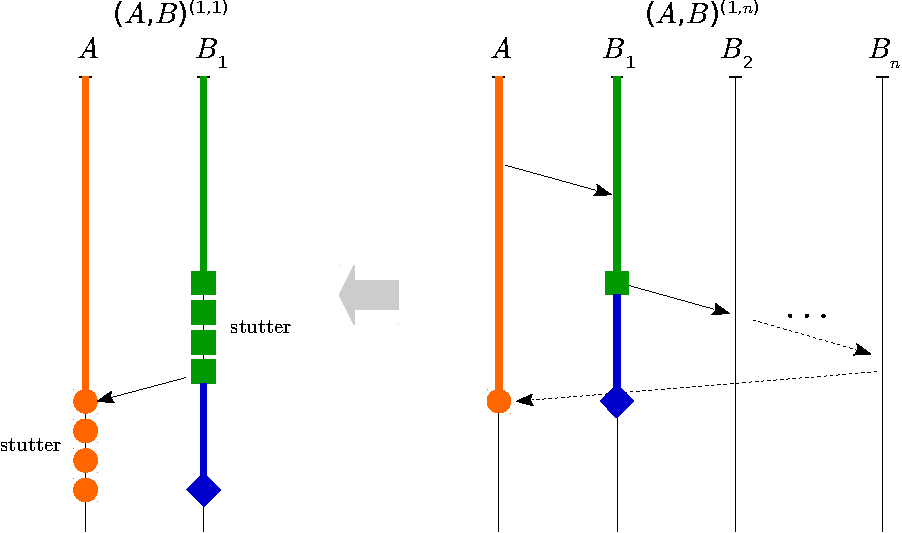
\includegraphics[scale=0.7]{token-systems/figures/simulation_proof}}
      \caption{Constructing a run of a cutoff system from a run of a large system.
        Vertical lines depict (local) paths of the processes,
        the horizontal lines mean the token transmission.
        The process $A$ starts with the token.%
      }
      \label{amba:fig:simulation_proof_1}
    \end{figure}
    We copy the behaviors of processes $A$ and $B_1$ until before $B_1$ sends the token.
    At this moment, we postpone sending the token by $B_1$ and stutter\footnote{
      To ``stutter a process $p$'' means ``not to schedule it''.
      As a result, a stuttered process neither reads inputs nor changes its state.
      In the figures it is shown by repeating a state.%
    }
    it,
    while the process $A$ continues execution until it gets into state \textcolor{orange}{$\CIRCLE$}
    ready to receive the token.
    Then $B_1$ transmits the token to process $A$.
    After that we move process $B_1$ into state \textcolor{blue}{$\blacklozenge$},
    while $A$ stutters in \textcolor{orange}{$\CIRCLE$}.
    Now we are in the original situation and repeat the construction.
    Since the property talks about process $A$ only, the resulting run satisfies it.
    Finally, we assumed that the processes of the large system pass the token infinitely often.
    If some process $B_x \in \{B_1,...,B_n\}$ holds the token forever,
    then we use its behavior for $B_1$ in the cutoff system
    (this may require to insert stuttering steps into behaviors of $B_1$ and $A$ of the cutoff system,
     to synchronize their (finitely many) token transmissions).

    Consider direction $\Leftarrow$. After contra-positioning:
    $$
    (A,B)^{(1,1)} \not\models \varphi(A) ~~\Rightarrow~~ \largesys \not\models \varphi(A).
    $$
    Given a system run of $(A,B)^{(1,n)}$ that satisfies $\neg\varphi(A)$,
    we build a system run of $(A,B)^{(1,1)}$ that satisfies $\neg\varphi(A)$.
    Figure~\ref{amba:fig:simulation_proof_2} shows how to construct a run of a system
    that has one more $B$ process than the cutoff system.
    By repeating the construction we can add the necessary $n-1$ $B$-processes.
    The construction works as follows.
    \begin{figure}[t]\centering{
      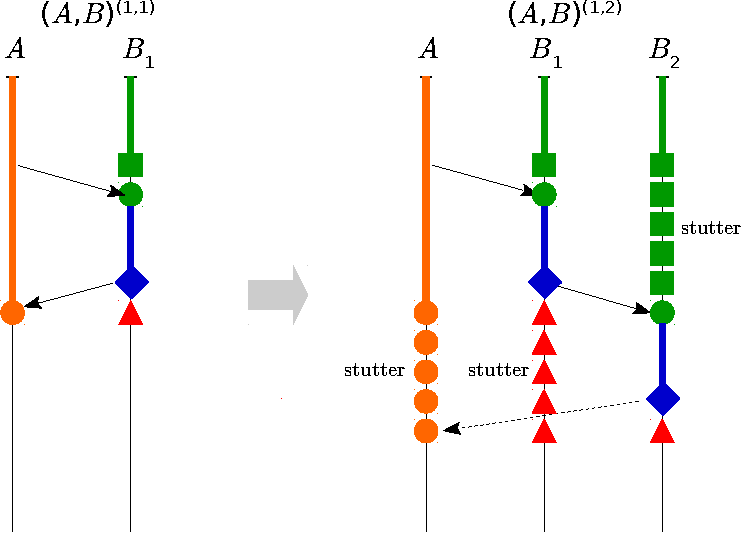
\includegraphics[scale=0.7]{token-systems/figures/simulation_proof2}}
      \caption{Constructing a run of a system $(A,B)^{(1,2)}$ from a run of a cutoff system $(A,B)^{(1,1)}$.
        Vertical lines depict (local) paths of the processes,
        the horizontal lines mean the token transmission.
        The process $A$ starts with the token.%
      }
      \label{amba:fig:simulation_proof_2}
    \end{figure}
    The new process $B_2$ copies the behavior of $B_1$ until before $B_1$ receives the token
    (i.e., up to the state \textcolor{green}{$\rule{0.6em}{0.6em}$}).
    Then it stutters in \textcolor{green}{$\rule{0.6em}{0.6em}$} awaiting for the token from process $B_1$.
    After that it copies $B_1$ behavior from state \textcolor{green}{$\CIRCLE$} till \textcolor{blue}{$\blacklozenge$},
    while processes $A$ and $B_1$ stutter.
    Then $B_2$ sends the token to $A$ and we return to the original situation.
    Finally, the case of $B_1$ or $A$ holding the token forever is straightforward.

    \parbf{Item (2)}
    Consider the case $\forall i. \varphi(B_i)$.
    First, we use the symmetry argument: for every $n$,
    $$
    \largesys \models \forall i.\varphi(B_i) ~\Iff~ \largesys \models \varphi(B_1).
    $$
    It holds because, for every $B_i$ and system run that satisfies $\neg\varphi(B_i)$,
    we can construct a run that satisfies $\neg\varphi(B_1)$.
    The latter is possible because all $B$-processes start without the token and $\varphi$ is 1-indexed%
    \footnote{%
      In contrast,
      the symmetry argument will not work for properties of the form $\forall i. \varphi(A,B_i)$,
      because $B_1$, $B_n$, and $B_{x \in \{2,...,n-1\}}$ have different ``relation'' to $A$.
      For example, take the formula $\forall i. \G(\token_A \impl \token_A \W \token_i)$.
      The (wrongly applied) symmetry argument would produce $\G(\token_A \impl \token_A \W \token_1)$,
      which says that the token moves from $A$ to $B_1$ (trivially true in every system),
      but the original formula does not hold.%
    }.

    After applying the symmetry argument,
    we can use the very same constructions as in item (1),
    see Figures~\ref{amba:fig:simulation_proof_1}~and~\ref{amba:fig:simulation_proof_2}.
    Let us only note the case when the token is stuck in some process.
    As for the construction in Figure~\ref{amba:fig:simulation_proof_2},
    this is simple: the token will be stuck in $A$ or in $B_1$ in the large system too.
    Consider the case in Figure~\ref{amba:fig:simulation_proof_1},
    when the token gets stuck in some process $B_d$ for $d \neq 1$.
    This is the only place in the proof where we use the peculiar structure of the formula to verify:
    $A^B_{loc,1} \land \GF\token_1 \impl \psi(B_1)$.
    Recall that the contra-position negates it and gives 
    $A^B_{loc,1} \land \GF\token_1 \land \neg \psi(B_1)$.
    Thus, in the large system the process $B_1$ receives the token infinitely often,
    and we can simply ignore the case\footnote{%
      We \emph{did} consider the case in other proof branches,
      to avoid relying on the peculiarity of the formula.
      We conjecture that in the case of (more general) properties of the form $\forall i. \varphi(B_i)$ (without $\GF\token_i$),
      the cutoff increases to $(1,2)$.%
    }.
  \end{proof}

  Let us note that without the assumption ``$A$ starts with token'' the constructions break.
  We conjecture that in this case a cutoff increases to $(1,2)$.

\subsection{Experiments} \label{amba:sec:experiments}

  In this section,
  we describe optimizations that are crucial for the synthesis of the parameterized AMBA,
  and present synthesis timings and resulting implementations.
  Most of the optimizations were already described in Section~\ref{tok_rings:sec:optimizations}.
  One interesting and not previously described optimization is ``Decompositional synthesis'',
  where the specification is synthesized incrementally, starting from a subset of the properties.
  It is this optimization that allowed us to synthesize the AMBA.

\parbf{Prototype}
  Our prototype is based on our tool \textsc{Party}~\cite{party},
  a synthesizer of parameterized token rings.
  \textsc{Party} is written in Python,
  uses LTL3BA~\cite{LTL3BA} for automata translation and Z3~\cite{Moura08} for SMT solving.
  The prototype and specification files can be found at \small{\url{https://github.com/5nizza/Party/}} (branch `amba-gr1').
  The experiments were run on a x86\_64 machine with $2.6$GHz CPU, $12$GB RAM, Ubuntu OS.

\parbf{Synchronous hub abstraction (Section~\ref{tok_rings:sec:optimizations})}
  Synchronous hub abstraction can be applied to 1-indexed specifications.
  It lets the environment simulate all but one process, and always schedules this process.
  Thus, the synthesizer searches for a process template in the synchronous setting
  with additional assumptions on the environment, namely: 
  (i) the environment sends the token to the process infinitely often, and
  (ii) the environment never sends the token to the process if it already has it.
  The synchronous hub abstraction is \emph{sound and complete} for 1-indexed properties.
  After applying this optimization \emph{any} monolithic synthesis method
  can be applied to the resulting specification
  (in the form of Eq.\ref{tok_rings:eq:hub-abstraction} on page~\pageref{tok_rings:eq:hub-abstraction}).

\parbf{Hardcoding states with and without the token~\cite[Section4]{Khalimov13}}
  The number of states with and without the token in a process template
  defines the degree of the parallelism in a token ring.
  Parallelism increases with the number of states that do not have the token.
  In the AMBA case study, any grants related action depends on having the token.
  Thus we divide the states in the process template:
  (a) one state does not have the token, while
  (b) all other states have the token.
  We do this by hardcoding the $\tok$ output function.

\parbf{Decompositional synthesis of different grant schemes}
  The idea of the decompositional synthesis is:
  synthesize a subset of the properties,
  then synthesize a larger subset using the model from the previous step as the basis.
  %   As will be noted in the experiments section, all previous optimizations still do not allow us to synthesize AMBA.
  %   It is a successive synthesis approach of properties together with hardcoding token states (next paragraph) that have made it.
  Consider an example of the synthesis of the non-0-process of AMBA.
  The flow is: 
  \begin{enumerate}
  \- Assume that every request is a locked request of type \hburstfour, i.e., 
     add the assumption $\always(\hlocki\land\hburst=\hburstfour)$ to the specification.
     This implicitly removes guarantee G2 and assumption A1 from the specification.
     Synthesize the model. The resulting model has $10$ states
     (states $t0,..,t9$ with their outputs, as well as transitions between them that satisfy the added assumption,
      are in Figure~\ref{amba:fig:ith-model}).

  \- Use the model found in the previous step as the basis:
     assert the number of states, values of output functions in these states, transitions for inputs that satisfy the previous assumption.
     Transitions for inputs that violate the assumption from step 1 are not asserted, and thus are left to be synthesized.

     Now relax the assumptions: allow locked and non-locked \hburstfour\ requests, i.e., replace the previous assumption with $\always(\hburst=\hburstfour)$.
     Again, this implicitly removes G2 and A1.
     In contrast to the last step, now guarantee G3 is not necessarily `activated' if there is a request.

     Synthesize the model.
     This may require increasing the number of states (and it does, in the case of non-0 process)---add new states and keep assertions on all the previous states.

  \- Assert the transitions of the model found, as in the previous step.\\
     Remove all added assumptions and consider the original specification.
     Synthesize the final model.
\end{enumerate}

Although for AMBA this approach was successful, it is not clear how general it is.
For example, it does not work if we start with locked \hburstfour\ and \hready\ always high,
and then try to relax it.
Also, the separation into sets of properties to be synthesized was done manually.

% 
\begin{figure}[t]\centering{
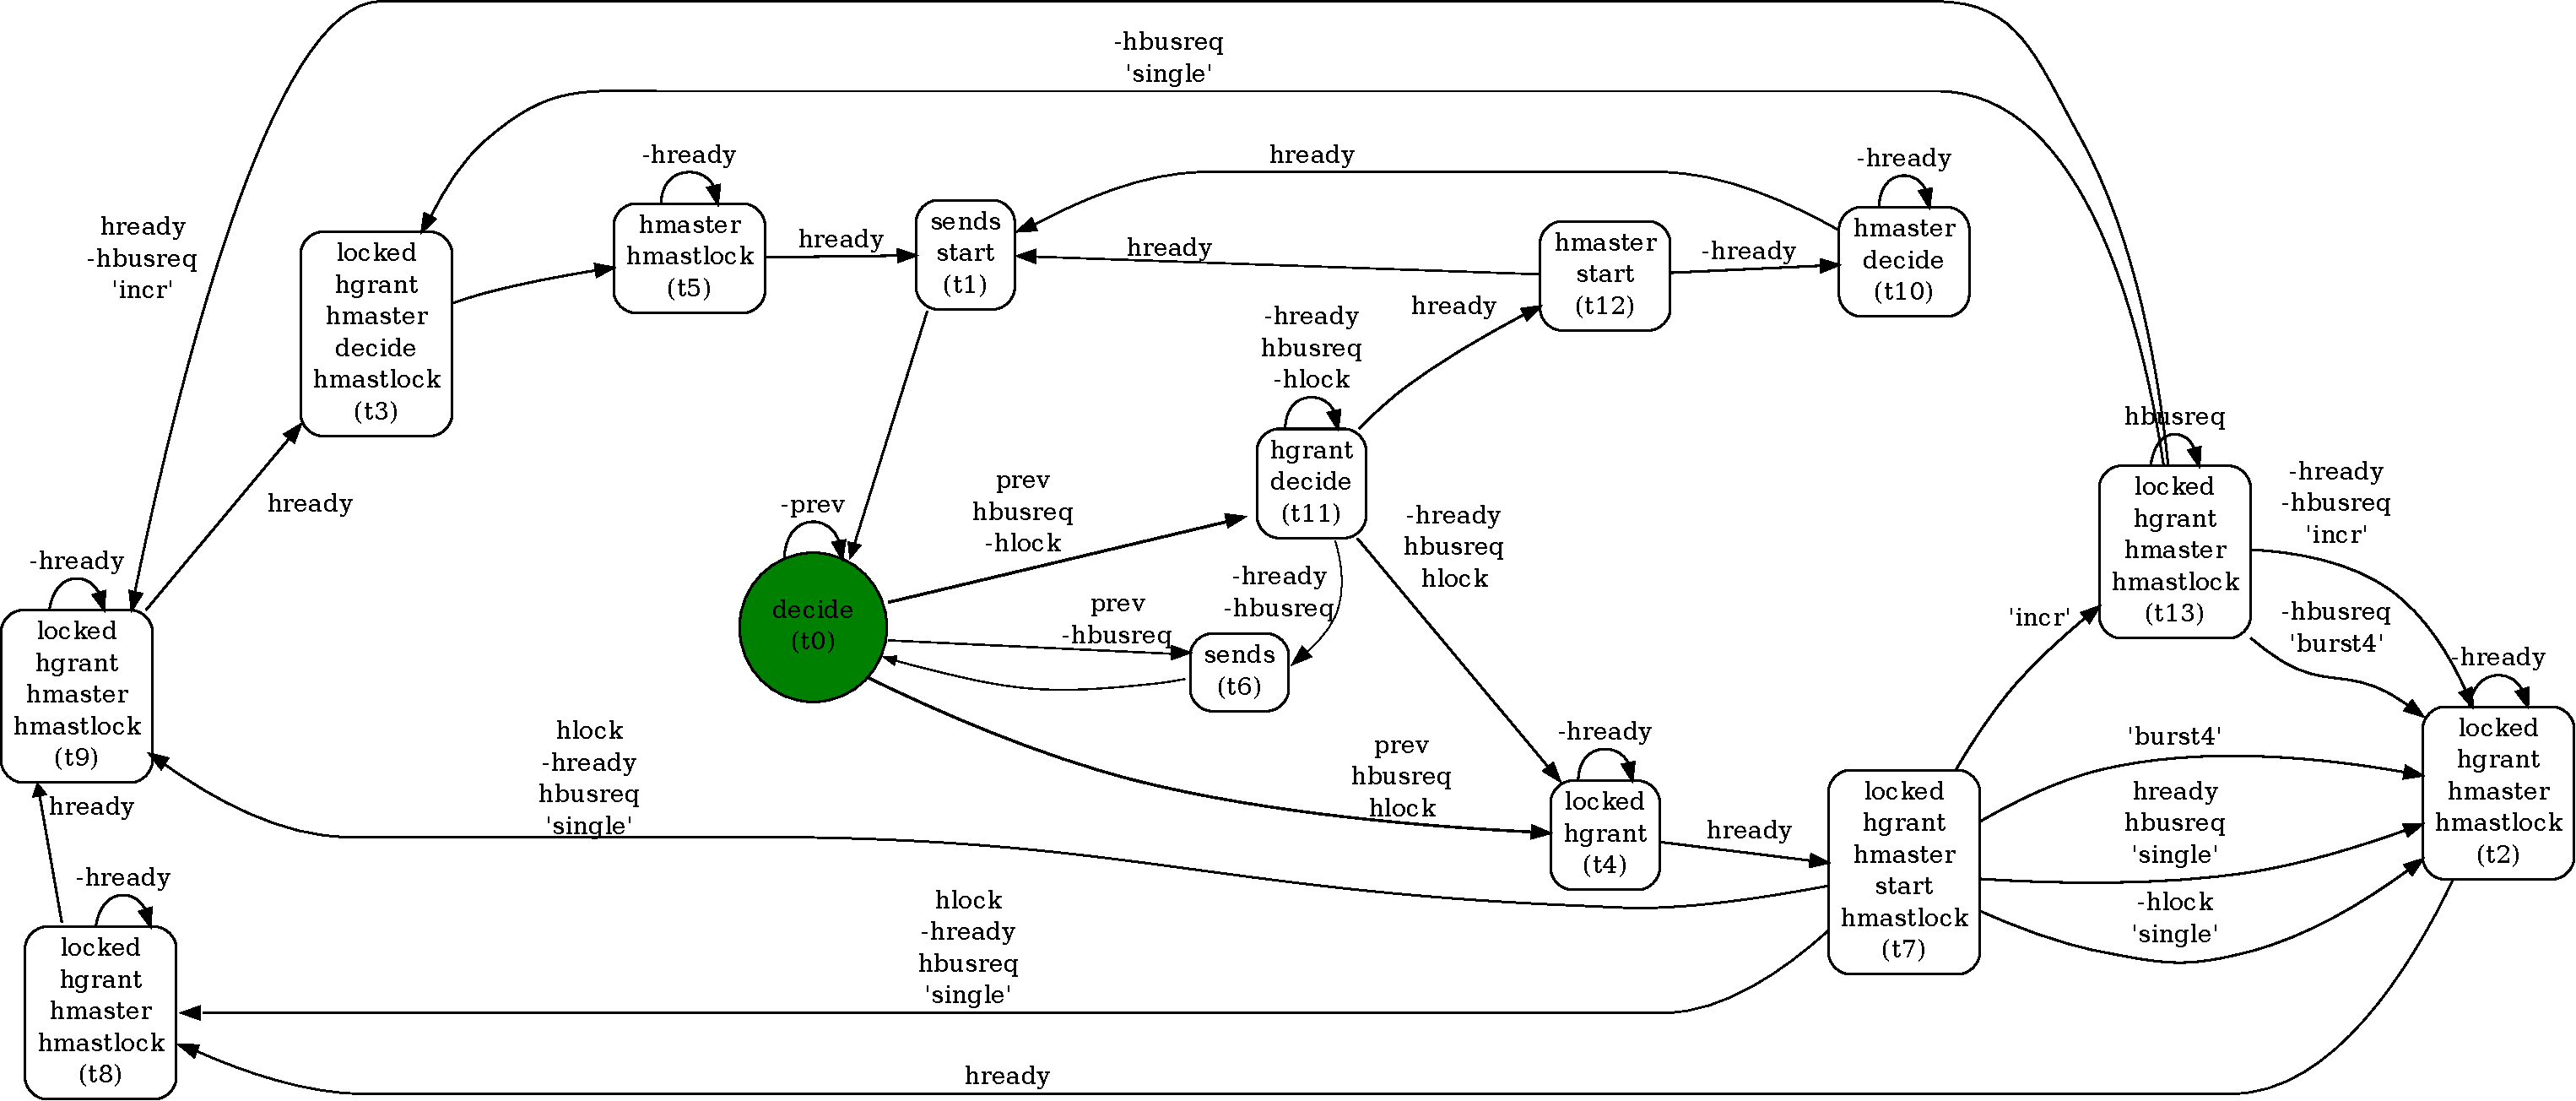
\includegraphics[width=\textwidth]{token-systems/figures/ith-model}}
\caption{Synthesized model of non-$0$-processes (after manual simplification).
Circle green state ($t0$) is without the token, other states are with the token.
The initial state is $t0$.
States are labeled with their active outputs.
Edges are labeled with inputs, a missing input variable means ``don't care''.
`Burst4' means $\hburst=\hburstfour$, `incr' means $\hburst=\hincr$, `single' means neither of them.
In the first step of decompositional synthesis states $t0,..,t9$ were synthesized, in the second $t10,..,t12$ were added, in the final step state $t13$ was added.}
\label{amba:fig:ith-model}
\end{figure}
%
\begin{figure}[t]\centering{
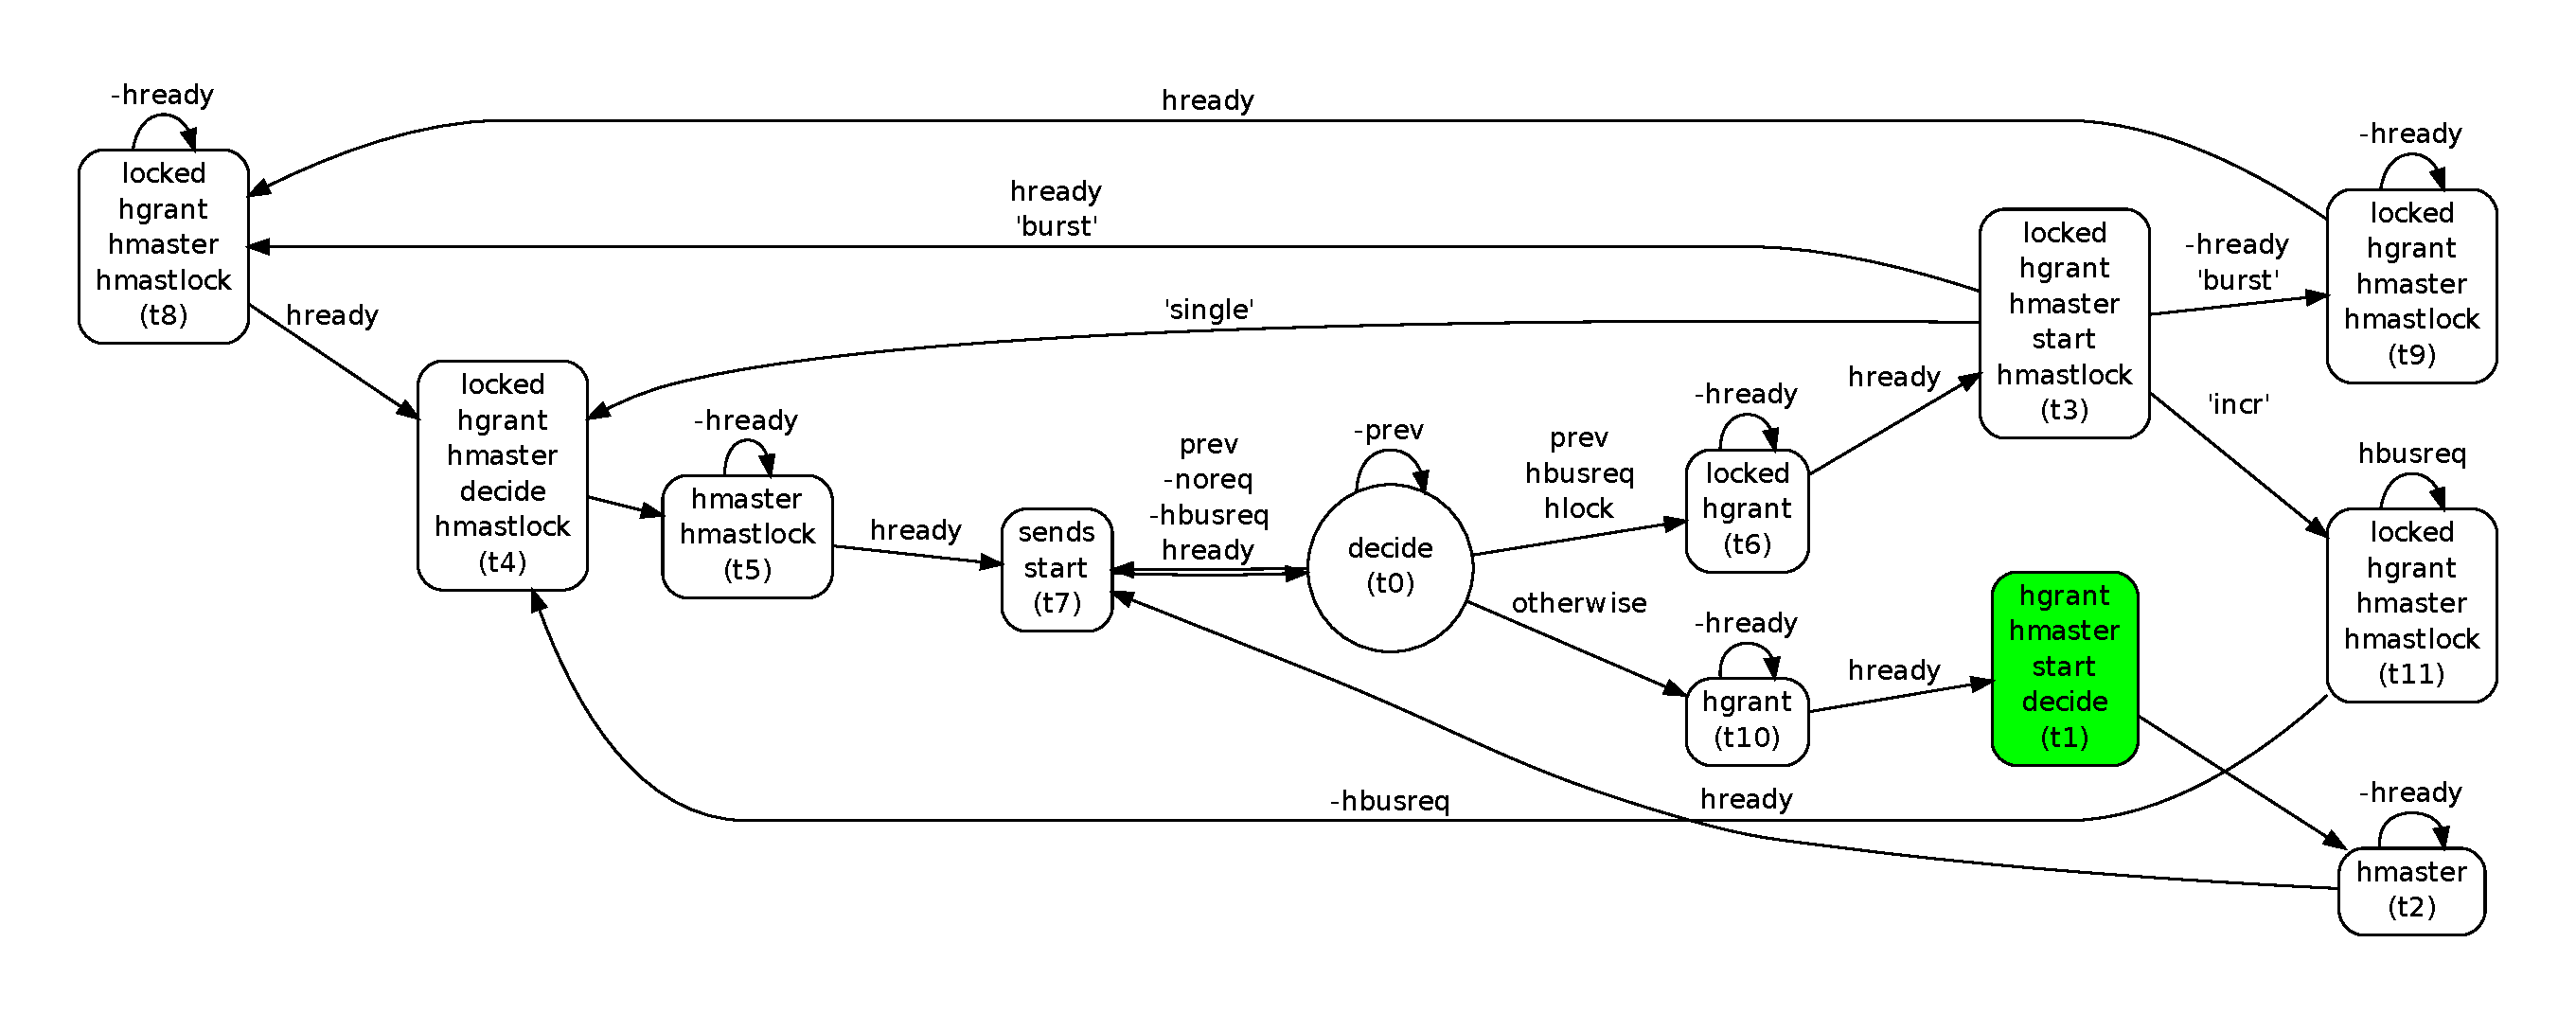
\includegraphics[width=\textwidth]{token-systems/figures/0-model}}
\caption{Synthesized model of $0$-processes (after manual simplification).
Circle state ($t0$) is without the token, other states are with the token.
The initial state is $t1$.
States are labeled with their active outputs.
Edges are labeled with inputs, a missing input variable means ``don't care''.
`Burst' means $\hburst=\hburstthree$ (recall we decreased the length of bursts for 0 process), `incr' means $\hburst=\hincr$, `single' means neither of them.
In the first step of decompositional synthesis states $t0,..,t10$ were synthesized, in the second only transitions were synthesized, but no new states added, in the final step $t11$ was added.}
\label{amba:fig:zero-model}
\end{figure}
%\todo{can we reuse ith models for the zero-process?}


%\parbf{Optimization of SMT Encoding}\label{sec:simpleGR1}
%%
%\newcommand{\Atm}{\ensuremath{{A_{\neg\varphi}}}}
%Recall from Section~\ref{sec:approach} that SMT based bounded synthesis, given an automaton \Atm\ of the negation of specification $\varphi$ and an unknown process template $P=(\Locals_P, \LocalsI, \ActionsProc, \delta_P, out)$ with a fixed number of states, encodes the product automaton $\Atm \times P$ into SMT constraints such that $\Atm \times P$ contains no reachable loops with an accepting state of the \Atm\ iff SMT constraints are satisfiable.
%Below is a general assertion from which the SMT query is composed: 
%$$
%\bigwedge{q\in Q_P}
%\bigwedge{\trans{a}{b}{i,o}\in \delta_\Atm}: \ \ \ 
%\rho(a,q) \ge 0 \land o=out(q) 
%\impl
%\rho(b,\delta_P(q,i)) 
%% 
%% [> \text{ if } b \text { is accepting, else } \ge] 
%\vartriangleright
%\rho(a,q)
%$$
%where $\vartriangleright$ is `$>$' if $b$ is an accepting state of \Atm, else `$\ge$'.
%In words: for any state of the process template, and any transition of the automaton, if the current state of the product automaton is reachable, then the next state should also be reachable and the ranking function should be as stated.
%
%The specification of AMBA we synthesize is derived from GR(1) specification.
%As a consequence it contain assumptions (A3, A6) of the form
%$\always\alpha(i)$ where $\alpha(i)$ is a Boolean formula over current inputs, and many guarantees (G1, G4, G5, G6, G7, G8, G12, G10.2) of the form $\always\beta(i,o,o')$ where $\beta(i,o,o')$ is a Boolean formula over current inputs and outputs and next outputs.
%Instead of using the standard approach via automaton translation described above, we:
%\begin{enumerate}
%  \item encode assertions of the form $\always\alpha(i)$ directly into SMT constraints, namely add $\alpha(i)$ to the the premise of the SMT rule. 
%  Thus, the premise becomes  
%  `$\rho(a,q)\ge 0 \land o=out(q) \mathbf{\land \alpha(i)} \impl ...$'
%
%  \item for all guarantees of the form $\always\beta(i,o,o')$ add SMT constraints of the form: 
%  $$
%  \bigwedge{q \in Q_P} \bigwedge{i \in \ActionsProc}: \ \ 
%  \alpha(i) \impl \beta(i,out(q),out(\delta_P(q,i)))
%  $$
%\end{enumerate}
%The first optimization is sound and complete, the second one: introduces incompleteness if used for model checking (since a given model may have unreachable state that violate the assertion), and seems to be complete for the synthesis.
%
%For AMBA specification in Figure~\ref{amba:fig:AMBAspecNewI} and \ref{amba:fig:AMBAspecNew0} this optimization means that only guarantees G2, G3, G9, G10.1, G11 require the standard flow via automata translation.
%
%Does this optimization help in the synthesis? 
%Preliminary experiments (considering the first step of the decompositional synthesis of non-0 process) show: 
%\begin{itemize}
%\item 
%With the optimization the automaton for the negated specification has 24 states, without -- 42 states.
%
%\item
%The synthesis time with optimization is 16 minutes, without -- 57 minutes.
%Interesting to note that the optimized and non-optimized versions spent the same time (2 minutes) checking satisfiability of the last query (with the model size of 10), so the main difference is in checking unsatisfiable queries -- Z3 identifies unsatisfiability of optimized queries faster (14 vs. 53 minutes).
%A similar behavior happens for a version of the same specification with reduced lengths of bursts ($3/4\impl 2/3$): total times are 3/6 minutes, but the last query took 1m40s/30s for optimized/non-optimized version. 
%
%\end{itemize}


%%%%%%%%%%%%%%%%%%%%%%%%%%%%%%%%%%%%%%%%%%%%%%%%%%%%%%%%%%%%%%%%%%%%%%%%%%%

\parbf{Results}
Synthesis times are in Tables~\ref{amba:tab:non-zero-process}~and~\ref{amba:tab:zero-process}, 
the model synthesized for non-0 process is in Figure~\ref{amba:fig:ith-model}.
The table has timings for the case when all optimizations described in this section are enabled --- it was not our goal to evaluate the optimizations separately, but to find a combination that works for the AMBA case study.

For the $0$-process we considered a simpler version with burst lengths reduced to 2/3 instead of the original 3/4 ticks.
With the original length, the synthesizer could not find a model within 2 hours (it hanged checking 11 state models, while the model has at least 12 states).

Without the decompositional approach,
the synthesizer could not find a model for for non-0 process of the AMBA specification within 5 hours.

\begin{table}[tb]
\footnotesize
\centering
\begin{minipage}[b]{0.45\textwidth}
\centering
% \setlength{\tabcolsep}{4pt}
\begin{tabular}{ l|cc }
Addit.\ assumptions                          & time & \#states \\
\hline
\rule{0pt}{3ex} \specialcellC{$\always \hlock$ \\ $\always \hburst=\hburstfour$} 
                       & 16min.  & 10  \\
\hline
\rule{0pt}{2ex} \specialcellC{$\always \hburst=\hburstfour$} & 13sec.  & 13  \\
\hline
\rule{0pt}{2ex} 
-- (Full Specification) & 1min.  & 14 \\
\end{tabular}
\caption{Results for non-$0$ process.\\~}
\label{amba:tab:non-zero-process}
\end{minipage}
% 
\hspace{0.5cm}
% 
\begin{minipage}[b]{0.45\textwidth}
\centering
% \setlength{\tabcolsep}{4pt}
\begin{tabular}{ l|cc }
Addit. assumptions & time & \#states \\
\hline
\rule{0pt}{3ex} \specialcellC{$\always \hlock$ \\ $\always \hburst=\hburstfour$} 
                       & 3h.  & 11  \\
\hline
\rule{0pt}{2ex} \specialcellC{$\always \hburst=\hburstfour$} & 1min.  & 11  \\
\hline
\rule{0pt}{2ex} 
-- (Full Specification) & 1m30s.  & 12 \\
\end{tabular}
\caption{Results for $0$-process \\ (bursts reduced: $3/4 \rightarrow 2/3$).}
\label{amba:tab:zero-process}
\end{minipage}
\end{table}

%\ak{`decide' is not faithfully simulated in token passing simulations?}


\subsection{Discussion}

We have shown that parameterized synthesis in token rings can be used to 
solve benchmark problems of significant size, in particular the well-known 
AMBA AHB specification that has been used as a synthesis benchmark for a long 
time. To achieve this goal, we slightly extended the cutoff results that 
parameterized synthesis is based on, and used a number of optimizations in 
the translation of the specification and the synthesis procedure itself to 
make the process feasible.

This is the first time that the AMBA case study, or any other realistic case,
has been solved by an automatic synthesis 
procedure for the parameterized case. However, some of the steps in the 
procedure are manual or use an ad-hoc solution for the specific problem at 
hand, like the limited extension of cutoff results for global inputs, the 
construction of suitable functions to convert local to global outputs, or the 
decompositional synthesis for different grant schemes. Generalizing and 
automating these approaches is a possible future work.

Our synthesized implementation is such 
that the size of the parallel composition grows only linearly with the number of 
components. Thus, for this case study our approach does not only solve the 
problem of increasing synthesis time for a growing number of components, but 
also the problem of implementations that need an exponential amount of memory 
in the number of components. We pay for this small amount of memory with a 
less-than-optimal reaction time, as processes have to wait for the token in 
order to grant a request. This restriction could be remedied by extending the 
parameterized synthesis approach to different system models, e.g., processes 
that coordinate by guarded transitions~\cite{EmersonK03},
or communicate via broadcast messages~\cite{EsparzaFM99}.



\section{Conclusion}\label{tok_rings:sec:conclusion}

In this chapter,
we studied the parameterized synthesis of token-ring systems from the applied perspective.
The starting point was the original approach of Bloem and Jacobs~\cite{JB14},
which could be applied only to toy specifications.
We suggested several optimizations that made
it applicable to larger ``made-up'' specifications.
Then we tackled the real-life specification, that of the AMBA bus protocol,
and suggested further optimizations.
This required us to extend the theory behind the approach.
In the end,
we synthesized a solution for the AMBA specification in the parameterized sense,
for the first time ever.
